\documentclass[journal=jctcce,manuscript=article,layout=traditional]{achemso}

\usepackage[T1]{fontenc}
\usepackage{amsmath,amssymb,bm}
\usepackage{booktabs}
\usepackage{graphicx}
\usepackage{tikz}
\usetikzlibrary{arrows.meta,positioning,fit,backgrounds}
\usepackage{xcolor}
\usepackage{url}

\setkeys{acs}{articletitle=true}
\newcommand{\vect}[1]{\bm{#1}}
\newcommand{\FACE}{\textup{\textsc{face}}}
\definecolor{faceblue}{HTML}{3a3a3a}
\definecolor{faceorange}{HTML}{3a3a3a}
\definecolor{muted}{HTML}{898781}

% Author details, shared by main.tex, si.tex and cover_letter.tex. Edit only this file.
\newcommand{\AuthorName}{Albert Linda}
\newcommand{\AuthorAffiliation}{Department of Materials Science and Engineering, Indian Institute of Technology Kanpur, Kalyanpur, Kanpur 208016, Uttar Pradesh, India}
\newcommand{\AuthorORCID}{0000-0002-3723-1756}
\newcommand{\AuthorEmail}{albert.hzbn@gmail.com}
\newcommand{\Funding}{This research received no specific grant from any funding agency in the public, commercial or not-for-profit sectors.}
\newcommand{\AuthorAddressLines}{Department of Materials Science and Engineering\\Indian Institute of Technology Kanpur\\Kalyanpur, Kanpur 208016, Uttar Pradesh, India}

\author{\AuthorName}
\affiliation{\AuthorAffiliation}
\email{albert.hzbn@gmail.com}

\title[Factorised Cartesian Cluster Expansion]{Factorised Cartesian Atomic Cluster Expansion for Low-Cost Machine-Learning Interatomic Potentials}

\begin{document}

\begin{abstract}
Machine-learning interatomic potentials can reach the accuracy of density functional theory at a fraction of its
cost, but the most accurate equivariant models remain expensive, mainly because of the tensor operations they perform
for every pair of neighbouring atoms. We present FACE, a factorised Cartesian atomic cluster expansion that removes
this bottleneck. Each neighbour contributes only a small set of radial functions and messages, and all mixing of
feature channels is done once per atom, so the cost per neighbour no longer grows with the size of the model. Custom
GPU kernels evaluate the remaining steps, and long-range electrostatics, dispersion and short-range repulsion can be
added through a single interface. We further show that training instabilities in this class of models originate in
how the network weights are scaled, and we introduce a distillation scheme in which an ensemble of models generates
additional, uncertainty-checked training data. On the rMD17 benchmark, with identical training budgets and hardware,
FACE matches the accuracy of a 128-channel MACE model on aspirin at an 11 times lower inference cost; compared with a
64-channel MACE it is 5.7 times faster, needs about four times less GPU memory and is more accurate on four of five
molecules. Training costs about the same per step. A distilled single model reaches energy and force errors of
2.26~meV and 6.74~meV/\AA{} on aspirin, close to the published MACE values (2.2 and 6.6), and runs stably in
molecular dynamics.
\end{abstract}

\begin{tocentry}
\centering
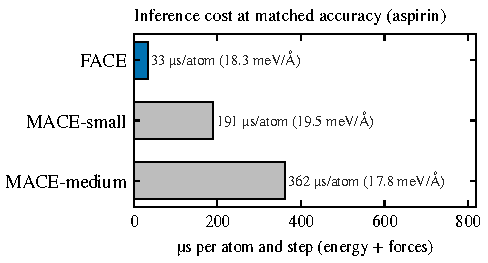
\includegraphics[width=3.25in]{figures/toc.pdf}
\end{tocentry}

%=====================================================================================================================
\section{Introduction}

Machine-learning interatomic potentials (MLIPs) predict the energy and forces of an atomic configuration. Their
accuracy approaches that of the electronic-structure method used to generate the training data, typically density
functional theory (DFT), while their cost is orders of magnitude lower\cite{behler2007,bartok2010gap}. They now underpin molecular-dynamics studies that are out of reach for
first-principles methods, and several reviews describe the state of the field\cite{unke2021chemrev,musil2021chemrev}.
Two developments define current practice. The first is to describe the environment of each atom by a body-ordered
expansion of its neighbour density, that is, by a sum of terms that each depend on the positions of a fixed number of
atoms (two-body, three-body and so on). Atom-centred symmetry functions\cite{behler2011sf}, the smooth overlap of atomic
positions (SOAP)\cite{bartok2013soap}, the spectral neighbour analysis potential (SNAP)\cite{thompson2015snap},
moment tensor potentials (MTP)\cite{shapeev2016} and the atomic cluster expansion
(ACE)\cite{drautz2019,dusson2022ace,lysogorskiy2021} can all be read as members or truncations of one such expansion.
ACE makes the construction systematic: a complete, body-ordered polynomial basis whose cost per atom is linear in
the number of neighbours. The second development is message passing, in which atoms exchange learned features with their neighbours over
several steps, so that each atom gradually sees a larger region. Invariant networks such as SchNet\cite{schutt2018schnet}, PhysNet\cite{unke2019physnet} and
DimeNet\cite{gasteiger2020dimenet} were followed by equivariant networks, whose internal features rotate
together with the structure: tensor field
networks\cite{thomas2018tfn}, PaiNN\cite{schutt2021painn}, NequIP\cite{batzner2022}, Allegro\cite{musaelian2023},
equivariant transformers\cite{liao2023equiformer,frank2022so3krates,wang2024visnet} and models with explicit
many-body messages such as QuinNet\cite{wang2023quinnet} and GotenNet\cite{aykent2025gotennet}. MACE\cite{batatia2022mace}
and graph ACE\cite{bochkarev2024grace} unify the two developments: they are ACE expansions whose density is built from
learned neighbour features, so that message passing increases the body order and the receptive field
together\cite{batatia2022botnet}.

On the revised MD17 (rMD17) benchmark\cite{chmiela2017md17,christensen2020rmd17}, the leading equivariant models now
differ by only a few meV/\AA{} in force error. The practical bottlenecks have therefore shifted from accuracy on small
molecules to cost, robustness and physics beyond locality. Four limitations motivate this work.

\emph{(i) Edge cost.} An atomic structure can be viewed as a graph whose edges connect neighbouring atoms. The
dominant cost of equivariant models is the tensor product computed on every edge, between the features of the
neighbour and the spherical harmonics of the bond direction. Its cost scales with the maximal angular momentum and
with the number of feature channels. SO(2) and Gaunt reductions\cite{passaro2023escn,luo2024gaunt} lower the
angular cost, and Cartesian formulations (MTP, TensorNet\cite{simeon2023tensornet}, CACE\cite{cheng2024cace},
irreducible Cartesian tensor products\cite{zaverkin2024ictp}) remove Clebsch--Gordan coefficients altogether. All of
them, however, keep channel-wide tensors on every edge, so that widening the model raises the dominant edge term.
Systematic cost--accuracy comparisons\cite{zuo2020benchmark} show that this trade-off, rather than the attainable
accuracy, often decides which potential is used in practice.

\emph{(ii) Long-range physics.} Local models cannot represent the total charge of a system or non-local charge
transfer. Long-distance equivariant features\cite{grisafi2019lode}, charge-equilibration networks such as
fourth-generation high-dimensional neural-network potentials\cite{ko2021}, models with explicit electronic
degrees of freedom\cite{unke2021spookynet}, Ewald message passing\cite{kosmala2023ewaldmp} and latent Ewald
summation\cite{cheng2024les} address this. The additional cost, and how such terms combine with a fast local model,
are rarely quantified.

\emph{(iii) Training robustness.} High-order polynomial features combined with normalisation layers can diverge. In
our experience and in published training recipes, this is usually handled by tuning learning rates and schedules
rather than diagnosed.

\emph{(iv) Data efficiency and uncertainty.} With about one thousand reference structures, single models overfit.
Deep ensembles\cite{lakshminarayanan2017} reduce the error and provide an uncertainty estimate but multiply the
inference cost. Knowledge distillation\cite{hinton2015distill} has been used to transfer the accuracy of large MLIPs
to small ones\cite{gardner2025distill,grace2025distill}; how the teacher's sampling should be restricted to the
region where the teacher is reliable has received less attention.

In this work we present \FACE{} (Factorised Cartesian Atomic Cluster Expansion). Its central idea is simple. In
current equivariant models, every edge carries a tensor as wide as the model itself, so a more expressive model is
proportionally more expensive on every edge. In \FACE{}, each edge carries only a few radial functions and a short
message; all widening happens once per atom, where it is cheap. We emphasise at the outset that \FACE{} belongs to the
ACE family. Its features are body-ordered contractions of neighbour-density moments, closely
related to MTP and to MACE's symmetric contractions, and Section~\ref{sec:aceequiv} makes this relation explicit.
The contributions are in how this expansion is parameterised, implemented and trained:
\begin{enumerate}
\item \emph{A cheaper edge.} A factorised edge density whose cost per edge does not depend on the model width, and
a variant based on a canonical-polyadic (CP) decomposition that restores separate radial functions for every
channel.
\item \emph{Cheap tensor messages and fused kernels.} Equivariant messages between message-passing steps are
computed by a single matrix multiplication followed by a fixed linear map, and custom GPU kernels evaluate the
pooling over neighbours and all per-atom algebra.
\item \emph{Pluggable physics.} One interface through which further energy terms are added, with their cost
measured: long-range electrostatics based on latent charges, with charge equilibration and smooth particle-mesh
Ewald summation (SPME)\cite{essmann1995spme}; dispersion; and the short-range repulsion of Ziegler, Biersack and
Littmark (ZBL).
\item \emph{Stable training.} A diagnosis of training divergence as a problem of how the weights are scaled, and a
fix (unit-variance parameterisation).
\item \emph{Better single models from ensembles.} A distillation scheme in which an ensemble of models (the
teacher) runs molecular dynamics, labels the visited structures on which its members agree, and trains a single
model (the student), which is finally fine-tuned on the DFT data alone; students join the next teacher
(``born-again'' iteration\cite{furlanello2018}).
\end{enumerate}
All comparisons with MACE that support efficiency claims use models trained on identical splits and epoch budgets
and timed on the same GPU; comparisons with published numbers are labelled as such.

The paper is organised as follows. Section~\ref{sec:background} summarises the atomic cluster expansion and its
message-passing form, and identifies where the cost arises. Section~\ref{sec:theory} derives the \FACE{} model, its
relation to ACE, the physics operators and a cost model, and Section~\ref{sec:training} describes the training
procedure and the distillation protocol.
Section~\ref{sec:implementation} describes the implementation, its extension points and the verification suite.
Section~\ref{sec:compdetails} gives the computational details, and Section~\ref{sec:results} reports accuracy
(including ablations, uncertainty and distillation), computational cost, training stability, long-range benchmarks
and molecular-dynamics tests.
Section~\ref{sec:discussion} discusses the position of \FACE{} among related models and its limitations.

%=====================================================================================================================
\section{Background: atomic cluster expansion and message passing}
\label{sec:background}
This section summarises the two ideas on which \FACE{} builds and shows where their computational cost arises.
Readers familiar with ACE and MACE can continue with Section~\ref{sec:theory}.

\subsection{Atomic cluster expansion}
In ACE\cite{drautz2019,dusson2022ace} the energy is a sum of atomic energies, $E=\sum_iE_i$, and each $E_i$ is
expanded in body-ordered features of the neighbour density of atom $i$. The one-particle basis is projected onto
the neighbourhood,
\begin{equation}
A_{i,znlm}=\sum_{j\in\mathcal N(i)}\delta_{z,Z_j}\,R_{nl}^{Z_iZ_j}(r_{ij})\,Y_{lm}(\hat{\vect r}_{ij}),
\label{eq:aceA}
\end{equation}
where $\mathcal N(i)$ are the neighbours within the cutoff $r_c$, $R_{nl}$ are radial functions and $Y_{lm}$
spherical harmonics. Products of $\nu$ such projections,
$\boldsymbol{A}_{i,\boldsymbol v}=\prod_{t=1}^{\nu}A_{i,v_t}$, are $(\nu+1)$-body functions of the environment,
because each projection is a single sum over neighbours. Rotation-invariant features $B_{i,\boldsymbol v}$ follow by
coupling the angular indices with generalised Clebsch--Gordan coefficients, and $E_i=\sum_{\boldsymbol v}
c_{\boldsymbol v}B_{i,\boldsymbol v}$ or a nonlinear function of the $B$. The essential computational property is
that the expensive many-body structure is formed per atom from the projections $A$, which cost only one sum over
neighbours. MTP\cite{shapeev2016} uses the same construction with Cartesian moment tensors
$\sum_jf_\mu(r_{ij})\,\hat{\vect r}_{ij}^{\otimes\nu}$ in place of $R_{nl}Y_{lm}$.

\subsection{Message passing as a learned density}
MACE\cite{batatia2022mace} replaces the fixed chemical index $z$ in Equation~\ref{eq:aceA} by learned neighbour features
$h_{j,k}$ with $k=1,\dots,C$ channels. In the first layer,
\begin{equation}
A^{(1)}_{i,klm}=\sum_jR^{(1)}_{kl}(r_{ij})\,Y_{lm}(\hat{\vect r}_{ij})\sum_{\tilde k}W_{k\tilde k}h^{(0)}_{j,\tilde k},
\end{equation}
and in later layers the neighbour features $h_j$ are themselves equivariant, so that the edge operation becomes a
channel-wise tensor product between $h_j$ and $Y(\hat{\vect r}_{ij})$ weighted by learned radial functions. A
symmetric contraction then forms body-ordered products per atom, as in ACE. The resulting cost has two parts. The
per-atom contraction scales with $C$ and with the correlation order. The per-edge tensor product scales with
$C$ multiplied by the number of coupling paths between the irreducible representations of $h_j$, $Y$ and the
output. For large systems the number of edges exceeds the number of atoms by the mean neighbour number $\bar M$,
typically 10--40, so the per-edge term dominates.

\subsection{Cartesian and spherical tensors}
A symmetric Cartesian tensor of rank $l$ has $(l+1)(l+2)/2$ independent components and decomposes into irreducible
parts of degree $l, l-2,\dots$: $\mathrm{Sym}^2(\mathbb R^3)=\mathbf 0\oplus\mathbf 2$ and
$\mathrm{Sym}^3(\mathbb R^3)=\mathbf 1\oplus\mathbf 3$. The symmetric powers $\hat{\vect u}^{\otimes l}$ of a unit
vector for $l=0,\dots,3$ therefore span the same function space as the spherical harmonics with $l\le3$, plus
redundant trace components that duplicate lower degrees. Cartesian models avoid Clebsch--Gordan coefficients because
contractions of Cartesian tensors are invariant whenever all indices are paired by Kronecker deltas. TensorNet,
CACE and ICTP use this property; MTP is its original form.

%=====================================================================================================================
\section{The \FACE{} model}
\label{sec:theory}

\subsection{Overview and notation}
\FACE{} computes the total energy as
\begin{equation}
E=\sum_i\Big[E^0_{Z_i}+s\sum_{t=1}^{T}\varepsilon_i^{(t)}\Big]+\sum_k\sum_iE_{k,i},
\label{eq:energy}
\end{equation}
where $E^0_Z$ are element reference energies, $s$ is a fixed output scale, $\varepsilon_i^{(t)}$ is the
atomic-energy contribution of message-passing step $t$ (we use $T=2$), and $E_{k,i}$ are per-atom energies of the
physics operators of Section~\ref{sec:physops}. Forces are $\vect F_i=-\partial E/\partial\vect r_i$ by automatic
differentiation, so the model is conservative by construction. Each atom carries scalar features
$\vect h_i^{(t)}\in\mathbb R^C$, initialised as a learned embedding of the element, $\vect h^{(0)}_i=\vect e_{Z_i}$.
Step $t$ performs four operations: (1) it builds Cartesian moments $A^{(l,t)}_i$, $l=0,\dots,3$, from the neighbours
(Sections~\ref{sec:moments}--\ref{sec:transport}); (2) it forms body-ordered invariants from the moments of all steps
so far (Section~\ref{sec:invariants}); (3) it updates the scalar features and emits $\varepsilon_i^{(t)}$; and (4) for
$t<T$ it forms equivariant vectors and matrices that are sent to the neighbours in the next step. Figure~\ref{fig:arch}
summarises the data flow, and Table~\ref{tab:notation} collects the symbols used below.

In plain terms, a single step works as follows. For every neighbour, the model computes a handful of numbers that
depend on the distance (radial functions) and a short summary of what the neighbour is (a message). These are
multiplied by simple polynomials of the bond direction and summed over all neighbours, giving a compact description
of the atom's surroundings. Everything that is expensive, such as mixing many feature channels and multiplying
descriptions together to capture three-, four- and five-body correlations, is then done once per atom rather than
once per neighbour. In the second step, atoms additionally send each other small vectors and matrices that describe
the orientation of their own environments.

\begin{table}
\caption{Main symbols and their values in the flagship configuration.}
\label{tab:notation}
\small
\begin{tabular}{lll}
\toprule
symbol & meaning & flagship \\
\midrule
$i$, $j$ & central atom, neighbour & \\
$r_{ij}$, $\hat{\vect u}_{ij}$ & distance and unit vector from $i$ to $j$ & \\
$r_c$ & cutoff radius & 4.5~\AA \\
$\bar n$ & mean number of neighbours in the training set & 12.3 (aspirin) \\
$Y_x$ & the 20 direction monomials of ranks $l=0$--3, Equation~\ref{eq:monomials} & \\
$B$ & number of learned radial functions $\phi_b$ per edge & 16 \\
$K$ & length of the neighbour message $m_{jk}$ & 32 \\
$C$ & node width (feature channels per atom) & 96 \\
$K_d$ & channels of the vectors $\vect V$ and matrices $\vect M$ sent between steps & 16 \\
$T$ & number of message-passing steps & 2 \\
$A^{(l)}_i$ & Cartesian moments (environment descriptors) of rank $l$ & \\
$P$, $Q$, $S$ & learned projections of the moments used in products & \\
$\vect h_i$ & scalar features of atom $i$ & \\
$\varepsilon_i^{(t)}$ & atomic energy contribution of step $t$ & \\
\bottomrule
\end{tabular}
\end{table}

\begin{figure}
\centering
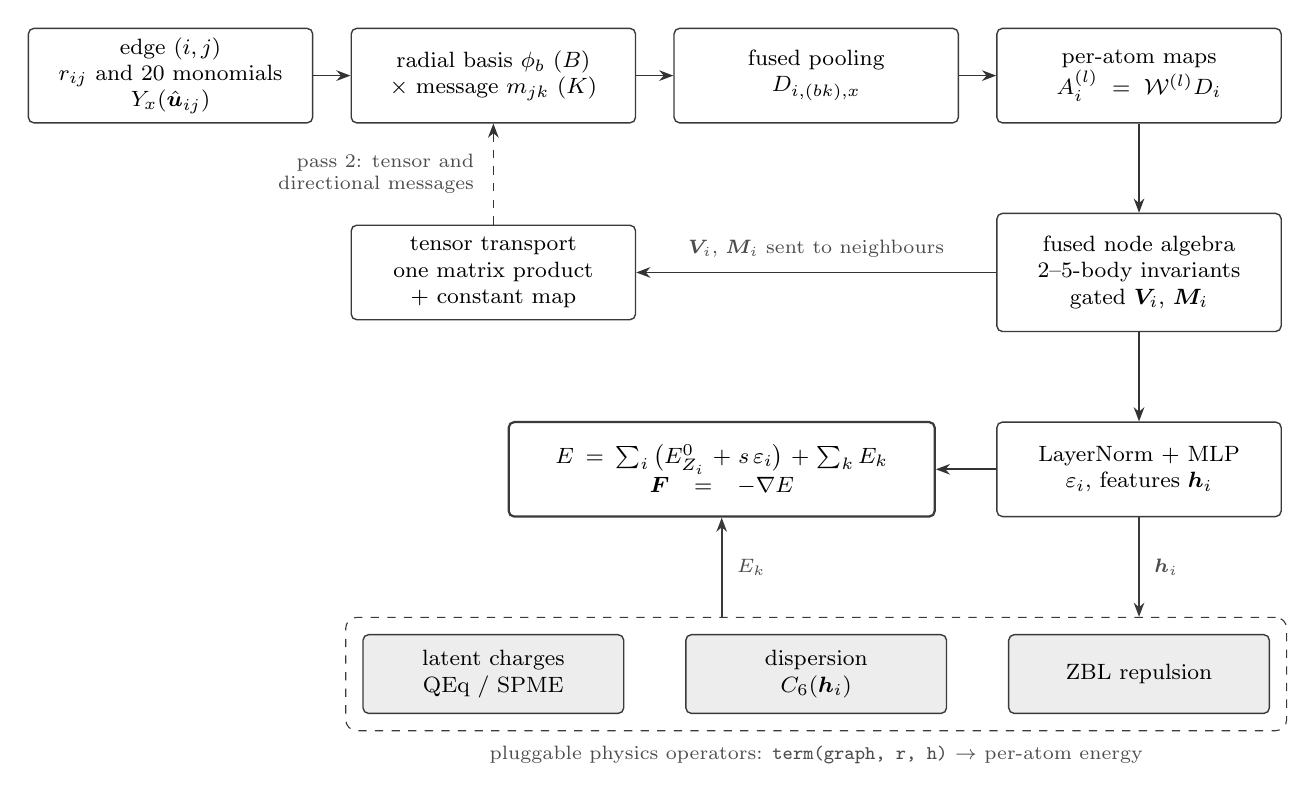
\begin{tikzpicture}[font=\footnotesize,
  box/.style={draw=faceblue, rounded corners=2pt, fill=white, line width=0.5pt, align=center, text width=34mm,
              execute at begin node={\hyphenpenalty=10000\relax},
              minimum height=12mm, inner sep=3pt},
  op/.style={draw=faceorange, rounded corners=2pt, fill=black!7, line width=0.5pt, align=center, text width=31mm,
             minimum height=10mm, inner sep=3pt},
  arr/.style={-{Stealth[length=1.8mm]}, line width=0.6pt, draw=black!80},
  lab/.style={font=\scriptsize, text=black!70, align=center, inner sep=1pt}]
% row 1: edge stage (left to right)
\node[box] (edge) at (0,0)    {edge $(i,j)$\\ $r_{ij}$ and 20 monomials\\ $Y_x(\hat{\vect u}_{ij})$};
\node[box] (fac)  at (4.1,0)  {radial basis $\phi_b$ ($B$)\\ $\times$ message $m_{jk}$ ($K$)};
\node[box] (pool) at (8.2,0)  {fused pooling\\ $D_{i,(bk),x}$};
\node[box] (mix)  at (12.3,0) {per-atom maps\\ $A^{(l)}_i=\mathcal W^{(l)}D_i$};
% row 2: node stage and transport (right to left)
\node[box, minimum height=15mm] (inv) at (12.3,-2.5) {fused node algebra\\ 2--5-body invariants\\ gated $\vect V_i$, $\vect M_i$};
\node[box] (trans) at (4.1,-2.5) {tensor transport\\ one matrix product + constant map};
% row 3: readout and total energy
\node[box] (mlp) at (12.3,-5.0) {LayerNorm + MLP\\ $\varepsilon_i$, features $\vect h_i$};
\node[box, fill=white, text width=52mm, line width=0.8pt] (E) at (7.0,-5.0)
     {$E=\sum_i\big(E^0_{Z_i}+s\,\varepsilon_i\big)+\sum_kE_k$\\[1pt] $\vect F=-\nabla E$};
% row 4: physics operators
\node[op] (es)   at (4.1,-7.6)  {latent charges\\ QEq / SPME};
\node[op] (disp) at (8.2,-7.6)  {dispersion\\ $C_6(\vect h_i)$};
\node[op] (zbl)  at (12.3,-7.6) {ZBL repulsion};
\begin{scope}[on background layer]
\node[draw=faceorange, dashed, rounded corners=4pt, inner sep=6pt, fit=(es)(disp)(zbl)] (ops) {};
\end{scope}
\node[lab, anchor=north, yshift=-1.5mm] at (ops.south) {pluggable physics operators: \texttt{term(graph, r, h)} $\to$ per-atom energy};
% arrows
\draw[arr] (edge) -- (fac);
\draw[arr] (fac) -- (pool);
\draw[arr] (pool) -- (mix);
\draw[arr] (mix) -- (inv);
\draw[arr] (inv) -- node[lab, above=1.5mm] {$\vect V_i$, $\vect M_i$ sent to neighbours} (trans);
\draw[arr, dashed] (trans) -- node[lab, left=2mm, align=right] {pass 2: tensor and\\ directional messages} (fac);
\draw[arr] (inv) -- (mlp);
\draw[arr] (mlp) -- (E);
\draw[arr, draw=faceorange] (mlp.south) -- node[lab, right=1.5mm] {$\vect h_i$} (mlp.south |- ops.north);
\draw[arr, draw=faceorange] (E.south |- ops.north) -- node[lab, right=1.5mm] {$E_k$} (E.south);
\end{tikzpicture}
\caption{Structure of \FACE{}. White boxes: local ACE-family model (one pass shown; the second pass adds directional
and tensor messages, dashed arrow). Grey boxes: pluggable physics operators, which receive the final features $\vect h_i$ and
add per-atom energies. The edge cost depends on $B$ and $K$ but not on the node width $C$.}
\label{fig:arch}
\end{figure}

\subsection{Local environment descriptors}
\subsubsection{Cartesian moments in symmetric storage}
\label{sec:moments}
For atom $i$ with neighbours $j$ within the cutoff $r_c$, let $\vect r_{ij}=\vect r_j-\vect r_i$,
$r_{ij}=|\vect r_{ij}|$ and $\hat{\vect u}_{ij}=\vect r_{ij}/r_{ij}$. Each direction is lifted to its symmetric
outer powers $\hat{\vect u}^{\otimes l}$, $l=0,\dots,3$, stored by their $1+3+6+10=20$ independent components
\begin{equation}
Y_x(\hat{\vect u})\in\{1;\ u_a;\ u_au_b\ (a\le b);\ u_au_bu_c\ (a\le b\le c)\},\qquad x=1,\dots,20.
\label{eq:monomials}
\end{equation}
Under a rotation or reflection $Q\in O(3)$, $\hat{\vect u}^{\otimes l}\mapsto Q^{\otimes l}\hat{\vect u}^{\otimes l}$,
so any linear map that acts only on channel indices commutes with $Q$ and preserves equivariance, and every full
index contraction of products is invariant. Compared with the 16 spherical harmonics with $l\le3$, the 20 monomials
contain four redundant trace components (the trace of the rank-2 tensor and the trace vector of the rank-3 tensor).
This redundancy is harmless for learning and avoids projections onto irreducible parts. Full tensors are formed only
per atom, where contractions are evaluated. Contractions in symmetric storage weight each component by its
multiplicity $w_x$ (1,1,1,2,2,2 for rank 2 and 1,1,1,3,\dots,3,6 for rank 3), e.g.\
$P^{(2)}\!:\!Q^{(2)}=\sum_xw_xP^{(2)}_xQ^{(2)}_x$. In words, the monomials $Y_x$ encode the direction of one bond up
to third order; summed over neighbours with suitable weights, they describe the angular shape of an environment, much
as a multipole expansion describes the shape of a charge distribution.

\subsubsection{Factorised edge densities}
\label{sec:factor}
Each edge carries two small objects. The first is a learned radial basis,
\begin{equation}
\phi_b(r_{ij};Z_i,Z_j)=\mathrm{MLP}\!\left[\,\mathrm{SiLU}\!\left(W\,\mathbf g(r_{ij})f_c(r_{ij})+\vect e_{Z_iZ_j}\right)\right]_b f_c(r_{ij}),\qquad b=1,\dots,B,
\label{eq:radial}
\end{equation}
with a multilayer perceptron (MLP), eight Bessel functions $\mathbf g$, the polynomial envelope $f_c$ of degree 6, an element-pair embedding
$\vect e_{Z_iZ_j}$ and SiLU activations\cite{elfwing2018silu}. The second is a low-rank neighbour message
$m_{jk}=(W_m\vect h_j)_k$, $k=1,\dots,K$, computed from the scalar features of the neighbour. The atomic density
\begin{equation}
D_{i,(bk),x}=\frac{1}{\bar n}\sum_j \phi_b(r_{ij})\,m_{jk}\,Y_x(\hat{\vect u}_{ij})
\label{eq:density}
\end{equation}
is a single batched matrix product of size $(BK)\times20$ per atom, where $\bar n$ is the mean number of neighbours
in the training set. The rank-$l$ moments with $C$ channels are obtained by channel maps that act per atom,
\begin{equation}
A^{(l)}_{i,c,x}=s_{Z_i,l,c}\sum_{b,k}\mathcal W^{(l)}_{c,(bk)}\,D_{i,(bk),x},\qquad x\in\text{rank }l,
\label{eq:channelmap}
\end{equation}
with a learned centre-element scale $s_{Z_i,l,c}$. The per-edge work is therefore $O(BK\cdot20)$ and independent
of $C$. In words, instead of giving every feature channel its own radial function on every edge, all channels share
$B$ radial functions and a $K$-component message; the per-atom map $\mathcal W^{(l)}$ then combines the pooled
products into as many channels as desired.

\subsubsection{Relation to the ACE density}
\label{sec:aceequiv}
Substituting Equation~\ref{eq:density} into Equation~\ref{eq:channelmap} gives
\begin{equation}
A^{(l)}_{i,c,x}=\frac{s_{Z_i,l,c}}{\bar n}\sum_j\mathcal R^{(l)}_c(r_{ij};Z_i,Z_j,\vect h_j)\,Y_x(\hat{\vect u}_{ij}),
\qquad
\mathcal R^{(l)}_c=\sum_{b=1}^{B}\sum_{k=1}^{K}\mathcal W^{(l)}_{c,(bk)}\,\phi_b(r_{ij};Z_i,Z_j)\,m_{jk}.
\label{eq:effradial}
\end{equation}
This is an ACE (or MACE) density, Equation~\ref{eq:aceA}, with a channel- and rank-dependent radial--chemical function
$\mathcal R^{(l)}_c$. In the first step $\vect h_j=\vect e_{Z_j}$, so $\mathcal R^{(l)}_c$ depends only on
$(r_{ij},Z_i,Z_j)$ and Equation~\ref{eq:effradial} is an ACE projection with a learned chemical embedding, as in
tensor-reduced ACE\cite{darby2022tensorreduced}. The factorisation restricts the $C$ functions $\mathcal R^{(l)}_c$
to a common $BK$-dimensional space spanned by products of $B$ radial functions and $K$ message components. This is
the source of the efficiency: the edge evaluates and pools the $BK$ basis products once, and the per-atom map
$\mathcal W^{(l)}$ produces any number of channels from them. It is also the main restriction: if the optimal
$\mathcal R^{(l)}_c$ need more than $BK$ independent combinations, accuracy is lost (Section~\ref{sec:ablation}).

\subsubsection{CP variant}
In \FACE-CP the map $\mathcal W^{(l)}$ is replaced by a canonical-polyadic (CP) decomposition\cite{kolda2009tensor}
of rank $C$, which is equivalent to per-(rank, channel) radial functions $R_{l,c}(r)$ multiplying a channel-wise
message $\mu_{jc}$,
\begin{equation}
A^{(l)}_{i,c,x}=\sum_{c'}\mathcal M^{(l)}_{cc'}\,\frac{s_{Z_i,l,c'}}{\bar n}\sum_j R_{l,c'}(r_{ij})\,\mu_{jc'}\,Y_x(\hat{\vect u}_{ij}),
\label{eq:cp}
\end{equation}
followed by a per-atom channel mixing $\mathcal M^{(l)}$. In words, the CP variant gives every channel its own
radial function again, which is more flexible but costs more per edge. This is the form of MACE's first-layer
density. The edge
cost is now $4C$ per edge and grows with $C$, but it is evaluated as one product of the 20 monomials with a
contiguous $(4C)$-wide edge tensor, keeping the rank-diagonal blocks of the small output.

\subsection{Messages between steps}
\subsubsection{Directional messages}
From the second step on, each atom also carries $K_d$ channels of equivariant vectors $\vect V_i$ and symmetric
matrices $\vect M_i$ (Section~\ref{sec:gated}). The scalar message is modulated by bond-projected invariants of both
end points,
\begin{equation}
m_{jk}\leftarrow m_{jk}+\big[W_d\,\vect d_{ij}\big]_k,\qquad
\vect d_{ij}=\big(\hat{\vect u}_{ij}\!\cdot\vect V_j,\ \hat{\vect u}_{ij}^{\top}\vect M_j\hat{\vect u}_{ij},\
\hat{\vect u}_{ij}\!\cdot\vect V_i,\ \hat{\vect u}_{ij}^{\top}\vect M_i\hat{\vect u}_{ij}\big),
\label{eq:directional}
\end{equation}
with one entry per channel $k\le K_d$, so $\vect d_{ij}\in\mathbb R^{4K_d}$. The angle between the bond and each
atom's own environment thus enters the second-step density without additional tensor products. All four entries
are invariant, so Equation~\ref{eq:density} remains equivariant.

\subsubsection{Tensor transport by a constant linear map}
\label{sec:transport}
Neighbours also send their equivariant tensors directly. The Cartesian analogues of the
$1\otimes0\to1$, $2\otimes1\to1$, $2\otimes0\to2$ and $1\otimes1\to2$ couplings of spherical models are
\begin{equation}
\sum_j\phi_b\vect V_j,\qquad \sum_j\phi_b\,\vect M_j\hat{\vect u}_{ij},\qquad \sum_j\phi_b\vect M_j,\qquad
\sum_j\phi_b\,\mathrm{sym}(\hat{\vect u}_{ij}\otimes\vect V_j),
\label{eq:transport}
\end{equation}
with $\mathrm{sym}(\vect a\otimes\vect b)_{ab}=\tfrac12(a_ab_b+a_bb_a)$. Optional rank-3 couplings add
$\sum_j\phi_b\,\mathrm{sym}(\hat{\vect u}\otimes\vect M_j)$ and
$\sum_j\phi_b\,\mathrm{sym}(\hat{\vect u}\otimes\hat{\vect u}\otimes\vect V_j)$. A naive implementation forms each
product on every edge. Instead, note that every term in Equation~\ref{eq:transport} is linear in the neighbour tensor
$T_j=[\vect V_j,\vect M_j]$ (9 components per channel) and polynomial of degree at most one in
$\hat{\vect u}$; for example $(\vect M_j\hat{\vect u})_a=\sum_{b}M_{j,ab}u_b$ and
$\mathrm{sym}(\hat{\vect u}\otimes\vect V_j)_{ab}=\tfrac12(u_aV_{j,b}+u_bV_{j,a})$. All of them are therefore fixed
linear combinations of the sums
\begin{equation}
S_{i,(p,b),(k,y)}=\frac{1}{\bar n}\sum_j Y_p(\hat{\vect u}_{ij})\,\phi_b(r_{ij})\,T_{j,k,y},\qquad
p\in\{1,u_x,u_y,u_z\},\quad y=1,\dots,9,
\label{eq:transportS}
\end{equation}
which is one batched matrix product of size $(4B)\times(9K_d)$ per atom. Every transport moment is then obtained by
a constant $(36\times18)$ matrix acting on the index pair $(p,y)$; its 18 outputs are the 3+3 vector and 6+6
matrix components of Equation~\ref{eq:transport}. With the rank-3 option, $p$ runs over the 10 monomials of degree
$\le2$ and the constant map is $(90\times38)$, adding two rank-3 outputs of 10 components each. The results are
mixed into the $C$ moment channels of the matching rank by per-atom maps from the $B\cdot2K_d$ (basis, channel)
pairs. No per-edge intermediate tensor is formed, and the map is verified against explicit per-edge evaluation to
$10^{-16}$ (Section~\ref{sec:verification}). In words, instead of forming several small tensor products on every
edge, the model sums each neighbour's vector and matrix weighted by distance and by the bond direction, and reads off
all required combinations afterwards from a fixed table of coefficients.

\subsection{Body-ordered invariants and readout}
\label{sec:invariants}
The moments describe the environment but still rotate with it. To obtain an energy, which must not change when the
structure is rotated, they are multiplied together and all Cartesian indices are summed out. Each resulting number
measures, for example, how strongly two directional features of the environment are aligned. In step $t$, the
moments of all steps $1,\dots,t$ are concatenated along the channel index. Per rank $l$, three
learned linear projections produce $P^{(l)}_{i,c}=\sum_{c'}W^{P,l}_{cc'}A^{(l)}_{i,c'}$ and similarly $Q^{(l)}$
and $S^{(l)}$, each with $C$ channels. Optionally, the projections are multiplied by centre-element-dependent gates
$g_{Z_i,l,c}$, which gives element-specific product weights as in MACE. The projections are contracted
channel-diagonally into nine invariant families (indices $a,b,d,e$ are Cartesian; channel index omitted):
\begin{align}
&\text{2-body:} && I_1=P^{(0)},\nonumber\\
&\text{3-body:} && I_2=P^{(1)}_aQ^{(1)}_a,\quad I_3=P^{(2)}_{ab}Q^{(2)}_{ab},\quad I_4=P^{(3)}_{abd}Q^{(3)}_{abd},\nonumber\\
&\text{4-body:} && I_5=P^{(1)}_aQ^{(2)}_{ab}S^{(1)}_b,\quad I_6=P^{(2)}_{ab}Q^{(2)}_{bd}S^{(2)}_{da},\quad
I_7=P^{(3)}_{abd}Q^{(2)}_{ab}S^{(1)}_d,\quad I_8=P^{(3)}_{abd}Q^{(3)}_{abe}S^{(2)}_{de},\nonumber\\
&\text{5-body:} && I_9=P^{(3)}_{abd}Q^{(1)}_aS^{(1)}_bQ^{(1)}_d,
\label{eq:invariants}
\end{align}
with summation over repeated indices. Each family is a full contraction with Kronecker deltas and hence invariant
under rotations. Under reflection, a rank-$l$ moment acquires the sign $(-1)^l$; the total rank of every family is
even (0, 2, 4, 6, 4, 6, 6, 8, 6), so all invariants are also parity-even and the energy is $O(3)$-invariant. In the
first step, each moment is a single sum over neighbours, so a product of $\nu$ moments is a $(\nu+1)$-body function
of the environment; this gives the body orders listed. The families are a subset of the ACE product basis up to
correlation order four with $l\le3$. They are not complete, and we make no completeness claim (see also
reference~\citenum{pozdnyakov2020}); the learned projections $P,Q,S$ supply the cross-channel couplings that a
channel-diagonal contraction alone would miss.

The $9C$ invariants are normalised by layer normalisation\cite{ba2016layernorm} and passed, together with the
current scalar features, to an MLP of widths $(9C+C)\to2C\to2C\to C+1$ (four further optional inputs are used only
with moment normalisation and are zero here). The first output is $\varepsilon_i^{(t)}$ and the remaining $C$
outputs update the features residually, $\vect h^{(t)}_i=\vect h^{(t-1)}_i+\Delta\vect h_i$.

\subsection{Gated equivariant products}
\label{sec:gated}
For the next step, each atom forms equivariant vectors and symmetric matrices from the same projections,
\begin{align}
\vect V&=a_0P^{(1)}+a_1\,Q^{(2)}S^{(1)}+a_2\,P^{(3)}\!:\!Q^{(2)}+a_3\,P^{(2)}Q^{(1)},\nonumber\\
\vect M&=\mathrm{sym}\big(b_0P^{(2)}+b_1\,P^{(1)}\!\otimes Q^{(1)}+b_2\,P^{(2)}Q^{(2)}+b_3\,P^{(3)}\!\cdot S^{(1)}\big),
\label{eq:gated}
\end{align}
with per-channel path weights $a_n$, $b_n$ (initialised to one), and multiplies them channel-wise by gates that are
linear functions of the invariants, $\vect V\leftarrow\vect g^V\odot\vect V$, $\vect g^V=W_gI+\vect 1$ (and
likewise for $\vect M$; $W_g$ is initialised to zero). The gated tensors are polynomials of degree up to three in
the moments. They are projected to $K_d$ channels for the directional messages and the transport of the next step,
so the body order of the second-step features grows multiplicatively with that of the first step, as in MACE.
Without these products, the transported tensors would be linear in the first-step moments and the second step would
add body order only through the scalar messages.

\subsection{Physics operators}
\label{sec:physops}
Every operator $E_k$ in Equation~\ref{eq:energy} has the same interface: it receives the graph, the interatomic
distances and the final scalar features $\vect h_i$, and returns per-atom energies. Forces follow by automatic
differentiation through the operator, including any linear solves.

\subsubsection{Latent-charge electrostatics}
A small MLP maps $\vect h_i$ to an electronegativity $\chi_i$ and a hardness $J_i=\mathrm{softplus}(\tilde J_i)
+0.1$~eV$/e^2$. Atoms carry Gaussian charges of width $\sigma=0.5$~\AA. Two such charges interact through the
smeared kernel $\mathrm{erf}(r/\gamma)/r$ with $\gamma=2\sigma$, which defines the Coulomb matrix $A_{ij}$
($A_{ii}=0$). The electrostatic energy is
\begin{equation}
E_\text{es}=\sum_i\chi_iq_i+\tfrac12\sum_iJ_iq_i^2+\tfrac12k_e\sum_{ij}q_iA_{ij}q_j,\qquad \sum_iq_i=Q,
\label{eq:qeq}
\end{equation}
with $k_e=14.3996$~eV\,\AA$/e^2$ and the total charge $Q$ of the structure as an input. In the \emph{coulomb} mode
the charges follow from a global chemical potential without Coulomb coupling,
\begin{equation}
q_i=-\frac{\chi_i-\mu}{J_i},\qquad \mu=\frac{Q+\sum_i\chi_i/J_i}{\sum_i1/J_i},
\end{equation}
which costs $O(N)$ and redistributes charge over the whole structure through $\mu$. In the \emph{qeq} mode the
charges minimise Equation~\ref{eq:qeq} including the Coulomb term (charge equilibration\cite{rappe1991qeq,ko2021}), which
requires the linear system
\begin{equation}
\begin{pmatrix}k_eA+\mathrm{diag}(\vect J)&\vect 1\\ \vect 1^\top&0\end{pmatrix}
\begin{pmatrix}\vect q\\ -\mu\end{pmatrix}=\begin{pmatrix}-\boldsymbol\chi\\ Q\end{pmatrix}.
\end{equation}
For periodic systems, $\tfrac12\vect q^\top A\vect q$ is evaluated by Ewald summation\cite{ewald1921} with a second
splitting width $\gamma'$,
\begin{equation}
\tfrac12\vect q^\top A\vect q=\tfrac12\sum_{i\ne j,\vect n}q_iq_j\frac{\mathrm{erf}(r/\gamma)-\mathrm{erf}(r/\gamma')}{r}
+\frac{2\pi}{V}\sum_{\vect k\ne0}\frac{e^{-\gamma'^2k^2/4}}{k^2}\big|S(\vect k)\big|^2
-\frac{1}{\sqrt\pi\gamma'}\sum_iq_i^2-\frac{\pi\gamma'^2}{2V}Q^2,
\label{eq:ewald}
\end{equation}
with $r=|\vect r_{ij}+\vect n|$ over lattice vectors $\vect n$, the structure factor
$S(\vect k)=\sum_iq_ie^{i\vect k\cdot\vect r_i}$ and a neutralising-background term for charged cells. We use
$\gamma'=\max(r_c/3.5,\,1.05\gamma)$, so that the real-space sum converges within the model cutoff and reuses its
neighbour list. The reciprocal sum is evaluated by SPME\cite{darden1993pme,essmann1995spme}: charges are spread on a
grid of spacing $\gamma'/4$ with order-4 cardinal B-splines, the grid is Fourier transformed, multiplied by the
Ewald kernel and the Euler-spline moduli, and the energy is accumulated, at a cost of $O(N+G\log G)$ for $G$ grid
points.

\subsubsection{Dispersion}
The dispersion operator is
\begin{equation}
E_\text{disp}=-\frac12\sum_{i\ne j}\frac{C_{6,ij}}{r_{ij}^6+R_{0,ij}^6}\,S(r_{ij}),\qquad
C_{6,ij}=\sqrt{C_{6,i}C_{6,j}},\quad C_{6,i}=C_{6,Z_i}^\text{free}\exp(\vect w\cdot\vect h_i),
\label{eq:disp}
\end{equation}
with free-atom $C_6$ coefficients and van der Waals radii $R_Z$ from Tkatchenko and Scheffler\cite{tkatchenko2009},
the geometric combination rule, rational Becke--Johnson-type damping\cite{grimme2011bj}
$R_{0,ij}=a_1(R_{Z_i}+R_{Z_j})/2+a_2$ with learned positive $a_1$, $a_2$, and a smooth switch $S$ that goes from one to
zero between 8 and 10~\AA. The environment modulation $\exp(\vect w\cdot\vect h_i)$ starts at one ($\vect w=0$) and
plays the role of the coordination dependence of D3\cite{grimme2010d3} or the Hirshfeld rescaling of TS. The sum
uses a separate pair list with a 10~\AA{} cutoff.

\subsubsection{Short-range repulsion}
The universal Ziegler--Biersack--Littmark (ZBL) potential\cite{ziegler1985zbl},
\begin{equation}
E_\text{ZBL}=\frac12\sum_{i\ne j}\frac{k_eZ_iZ_j}{r_{ij}}\,\varphi\!\left(\frac{r_{ij}}{a_{ij}}\right)S_\text{Z}(r_{ij}),
\qquad a_{ij}=\frac{0.4685~\text{\AA}}{Z_i^{0.23}+Z_j^{0.23}},
\end{equation}
with the standard four-exponential screening function $\varphi$, is switched off between 0.6 and 1.2~\AA{} by
$S_\text{Z}(r)=1-t^3(10-15t+6t^2)$, $t=(r-0.6~\text{\AA})/0.6~\text{\AA}$, which is $C^2$-continuous. It only acts at
distances that are not sampled in typical training data and prevents unphysical attraction there.

\subsection{Cost model}
\label{sec:costmodel}
Let $N$ be the number of atoms and $\bar M$ the mean number of neighbours. Table~\ref{tab:costmodel} lists the
multiply--add operations per edge and per atom of one second-step pass of the flagship ($C=96$, $B=16$, $K=32$,
$K_d=16$). The per-edge work, about $2.7\times10^4$ operations, is independent of $C$; it consists of the radial
network, the density product and the transport product. The per-atom work is proportional to $C$ and consists of
dense matrix products: the channel maps $\mathcal W^{(l)}$, the projections, the transport mixing and the readout
MLP. Counted in operations, both parts are of similar size at the 36 neighbours per atom of our condensed timing
boxes. They differ in hardware efficiency. The per-atom maps are large dense matrix products, which GPUs execute
efficiently, whereas edge operations involve gathers and irregular memory access and are bound by
memory bandwidth. Widening the model therefore raises only the efficient part of the cost: doubling $C$ from 64 to
128 increased the measured time by 29\% at 4.5k atoms, whereas the same change in MACE (MACE-small to
MACE-medium) increased it by 89\% (Table~\ref{tab:speed}); Section~\ref{sec:widthmem} measures this over a wider
range of widths. Memory follows the same pattern; the widest per-edge tensors are $BK$ (pooled inside the fused
kernel without being stored) and $9K_d$.

\begin{table}
\caption{Multiply--add operations of one second-step pass of the flagship ($C=96$, $B=16$, $K=32$, $K_d=16$). The
first step has no directional or transport terms.}
\label{tab:costmodel}
\small
\begin{tabular}{llr}
\toprule
operation & size & operations \\
\midrule
\multicolumn{3}{l}{\emph{per edge (independent of $C$)}} \\
radial network, Equation~\ref{eq:radial} & $8\to64\to64\to B$ & $5.6\times10^3$ \\
density product, Equation~\ref{eq:density} & $B\cdot K\cdot20$ & $1.0\times10^4$ \\
directional invariants, Equation~\ref{eq:directional} & $2\cdot9K_d+4K_d\cdot K$ & $2.3\times10^3$ \\
transport product, Equation~\ref{eq:transportS} & $4B\cdot9K_d$ & $9.2\times10^3$ \\
total per edge & & $2.7\times10^4$ \\
\midrule
\multicolumn{3}{l}{\emph{per atom ($\propto C$)}} \\
channel maps, Equation~\ref{eq:channelmap} & $BK\cdot C\cdot20$ & $9.8\times10^5$ \\
projections $P,Q,S$ & $2C\cdot3C\cdot20$ & $1.1\times10^6$ \\
transport mixing & $2K_dB\cdot C\cdot9$ & $4.4\times10^5$ \\
invariants and gated products & & $\approx3\times10^4$ \\
readout MLP & $10C\to2C\to2C\to C$ & $2.4\times10^5$ \\
\bottomrule
\end{tabular}
\end{table}

%=====================================================================================================================
\section{Training and distillation}
\label{sec:training}
This section describes how the models are trained, why the weights are parameterised as they are, and the
distillation protocol that turns an ensemble of models into a better single model.

\subsection{Reference energies and output scaling}
For single-molecule data sets the mean training energy is subtracted in
double precision before training in single precision; for data with varying composition, element reference energies
$E^0_Z$ are obtained by least squares on the training set. The output scale $s$ in Equation~\ref{eq:energy} is the
standard deviation of the training force components, and $\bar n$ is the mean neighbour number of the training set
(12.3 for aspirin at $r_c=4.5$~\AA).

\subsection{Loss and optimisation}
The loss is
\begin{equation}
\mathcal L=w_E\Big\langle\Big(\frac{E-E^\text{ref}}{N}\Big)^2\Big\rangle+w_F\big\langle|\vect F_i-\vect F_i^\text{ref}|^2\big\rangle
\end{equation}
with $(w_E,w_F)=(1,1000)$ for the first 75\% of epochs and $(1000,100)$ afterwards. We use Adam\cite{kingma2015adam}
with the AMSGrad correction\cite{reddi2018amsgrad} and decoupled weight decay (set to zero)\cite{loshchilov2019adamw},
a one-cycle learning-rate schedule\cite{smith2017onecycle} with peak 0.04, batch size 5, gradient-norm clipping at
10 and an exponential moving average (EMA, decay 0.99) of the parameters and of all buffers, which must be copied
explicitly. Training with forces requires second derivatives, because the loss depends on
$\partial E/\partial\vect r$; the model is therefore built from twice-differentiable operations.

\subsection{Unit parameterisation}
Every linear layer stores weights $W\sim\mathcal N(0,1)$ and applies the factor
$1/\sqrt{n_\text{in}}$ in the forward pass, $\vect y=W\vect x/\sqrt{n_\text{in}}+\vect b$, as in
e3nn\cite{geiger2022e3nn} and related parameterisation analyses\cite{yang2022mup}. The function at initialisation is
the same as with the default initialisation, which stores $W$ at scale $1/\sqrt{n_\text{in}}$ directly. The
difference lies in the optimiser dynamics. Adam normalises each update by a running estimate of the gradient
magnitude, so that the step on a stored weight is of order the learning rate $\eta$, independent of the gradient
scale. With the default parameterisation the relative change of an effective weight per step is therefore
$\eta/(1/\sqrt{n_\text{in}})=\eta\sqrt{n_\text{in}}$, which grows with the layer width: for the 1024-wide edge maps
and $\eta=0.01$ it is about 30\%. With unit parameterisation the relative change is $\eta$ for every layer. Wide
layers in this model sit directly before high-order polynomial products, which amplify relative changes of the
moments by up to the fifth power. Section~\ref{sec:stability} shows that this explains the divergences we observed.

\paragraph{Recovery from non-finite steps.} After 20 consecutive steps with a non-finite loss or gradient, the weights are restored from
the EMA, the optimiser state is reset and the learning rate is halved.

\subsection{Uncertainty-gated ensemble distillation}
\label{sec:distill}
An ensemble of $M_\text{T}$ independently trained models serves as teacher. For a configuration $\vect x$, the
teacher prediction is the member mean, and its uncertainty is the force spread
\begin{equation}
\sigma_F(\vect x)=\frac{1}{3N}\sum_{i,a}\mathrm{std}_m\big[F^{(m)}_{ia}(\vect x)\big],
\end{equation}
the standard deviation over members averaged over atoms and Cartesian components. The protocol is:
\begin{enumerate}
\item \emph{Teacher dynamics.} All training structures are propagated simultaneously by Langevin dynamics
(BAOAB splitting scheme\cite{leimkuhler2013baoab}, time step 0.5~fs, 400 steps, $T=500$~K) with the ensemble-mean forces.
\item \emph{Labelling and gating.} Every 20 steps, snapshots are labelled with the ensemble-mean energy and forces.
Snapshots with $\sigma_F$ larger than three times the mean spread on held-out data are discarded.
\item \emph{Student training.} A student is trained on the DFT data, repeated four times per epoch, together with the
teacher data, using the same number of optimiser steps as a 400-epoch run on DFT data alone.
\item \emph{DFT-only fine-tune.} The student is fine-tuned on DFT data only (60 epochs, peak learning rate
$4\times10^{-3}$), and optionally once more with an energy-weighted loss ($w_E=1000$, $w_F=10$, peak learning rate
$2\times10^{-3}$).
\item \emph{Iteration.} Students join the next teacher (``born-again'' iteration\cite{furlanello2018}); existing
teacher-MD configurations are relabelled by the new teacher.
\end{enumerate}
No additional DFT calculations are performed, and test structures are never used. The gate in step 2 matters
because the teacher's accuracy is only known on configurations similar to the training data; the threshold of three
times the test-set spread keeps the teacher data within this region (Section~\ref{sec:distillresults}). The final
DFT-only fine-tune removes any systematic bias that the teacher labels introduce. Distillation of MLIPs is
established\cite{hinton2015distill,gardner2025distill,grace2025distill}; the elements we add are the thermal
teacher-MD sampling with an uncertainty gate, iterated teachers, and the final DFT-only and energy-weighted
fine-tunes.


%=====================================================================================================================
\section{Implementation}
\label{sec:implementation}

\subsection{Software design and extension points}
\FACE{} is implemented in PyTorch\cite{paszke2019pytorch}, with CUDA kernels compiled at run time through
CuPy\cite{okuta2017cupy} and NVIDIA's run-time compiler (NVRTC), so that no host C++ compiler is needed. The model is one module whose components
are selected by constructor arguments and switches (Table~\ref{tab:options}); all switches are covered by the test
suite. Configurations differ only in these settings, so the flagship, the CP variant and the ablations of
Section~\ref{sec:ablation} are produced by the same code.

Physics operators are \texttt{torch.nn.Module} objects with the method \texttt{forward(graph, r, h)} that returns a
per-atom energy (Figure~\ref{fig:arch}). Adding an operator requires implementing this one method and registering its
name; the dispersion operator, for example, is 48 lines including its parameter tables. Because forces come from
automatic differentiation of the total energy, no force code is written for new operators. Operators that need
pairs beyond the model cutoff, such as dispersion, request a separate long-range pair list from the data pipeline.
Charges are written back to the graph, so later operators or analyses can use them.

For simulations, an ASE\cite{larsen2017ase} calculator wraps a trained model, and an ensemble calculator returns the
member mean together with per-atom force spreads. Trained checkpoints store the model configuration, the
reference energies and the normalisation constants, so a model is restored from one file.

\begin{table}
\caption{Model options. All combinations used in this work are produced by the same code.}
\label{tab:options}
\small
\begin{tabular}{lll}
\toprule
option & effect & default (flagship) \\
\midrule
\texttt{factor}, $B$, $K$ & factorised edge density, Equations~\ref{eq:density}--\ref{eq:channelmap} & on, 16, 32 \\
\texttt{cp} & CP density, Equation~\ref{eq:cp} & off \\
\texttt{transport} & tensor transport, Equation~\ref{eq:transport} & on \\
\texttt{transport3} & rank-3 transport couplings & off \\
\texttt{eqmsg} & gated equivariant products, Equation~\ref{eq:gated} & on \\
\texttt{elem\_proj} & element-dependent product gates & off \\
\texttt{max\_body} & truncate invariant families by body order & 5 \\
\texttt{poly\_readout} & linear readout in all but the last step & off \\
\texttt{terms} & physics operators: \texttt{coulomb}, \texttt{qeq}, \texttt{disp}, \texttt{zbl} & none \\
\texttt{fuse}, \texttt{compile\_radial} & fused kernels and spline radial tables (inference) & on for MD \\
\bottomrule
\end{tabular}
\end{table}

\subsection{Neighbour lists and batching}
Graphs are stored as a padded neighbour matrix of shape $N\times M_\text{max}$ with a mask and lattice shift
vectors, built with the ASE neighbour list. This layout makes every per-edge operation a dense tensor operation and
turns the pooling of Equations~\ref{eq:density} and~\ref{eq:transportS} into batched matrix products over the neighbour
dimension. Several structures are batched by concatenating their atoms. For the Coulomb operator of molecular
structures, the Coulomb matrix of a batch is block-diagonal, and the charge-equilibration systems of all structures
in a batch are solved together.

\subsection{Fused GPU kernels}
Two custom kernels implement the parts of the model that dominated the profile of the PyTorch implementation.

\emph{Density kernel.} The forward kernel evaluates Equation~\ref{eq:density} with one thread block per atom and one
thread per $(b,k)$ pair. Tiles of $\phi$, $m$ and $Y$ for consecutive neighbours are staged in shared memory, and
each thread accumulates its 20 monomial components in registers. The per-edge tensor of size $BK$, which dominated
the memory traffic of the PyTorch version, is never stored. The backward kernel keeps the gradient of one atom's
density in shared memory, forms per edge $T_{bk}=\sum_xG_{x,bk}Y_x$ once and reuses it for the gradients with
respect to $\phi$, $m$ and $Y$. It is organised in three tiled phases with padding against shared-memory bank
conflicts.

\emph{Node-algebra kernel.} One thread per (atom, channel) evaluates all nine invariant families of
Equation~\ref{eq:invariants} and the gated-product paths of Equation~\ref{eq:gated} directly from symmetric storage, holding the
full tensors in registers. Its backward pass folds the gradients of the full tensors back onto the symmetric
components.

Both kernels support first derivatives only. They are therefore used for inference and molecular dynamics, where
forces need one backward pass, whereas training, which needs second derivatives, uses the PyTorch path. The two
paths compute the same function to within $1.4\times10^{-6}$ (relative, float32). For inference, the learned radial
functions can also be tabulated per element pair (4096 points, cubic Hermite interpolation), and the complete
energy-and-force evaluation can be captured as a CUDA graph to remove kernel-launch overhead for small systems.

\subsection{Verification}
\label{sec:verification}
The test suite checks, in float64: invariance of $E$ and equivariance of $\vect F$ under rotations, reflections,
translations and permutations (to $10^{-9}$); forces against finite differences ($10^{-6}$ relative), including
through the charge-equilibration solve and Ewald sums; finite second derivatives, which force training requires;
$C^1$ continuity of energy and forces at $r_c$; lattice-translation invariance and exact supercell extensivity for
periodic cells; the NaCl Madelung energy ($2\times10^{-6}$ relative for two Ewald splittings); SPME against exact
Ewald ($3\times10^{-4}$ relative in energy, with the expected $h^4$ convergence in the grid spacing $h$); the transport
maps against explicit per-edge evaluation; and the fused kernels against the PyTorch path (outputs and all gradients
to $\le1.4\times10^{-6}$ relative).

%=====================================================================================================================
\section{Computational details}
\label{sec:compdetails}
\subsection{Data sets}
rMD17\cite{christensen2020rmd17} (PBE/def2-SVP). We use the official split 1: the 1000 training
indices of split 1 (file \texttt{index\_train\_01}) are shuffled with a fixed seed into 950 training and 50
validation structures, and the 1000 test indices (\texttt{index\_test\_01}) form the test set, which is used only for
final evaluation. Energy errors are for total energies of the molecule (meV per structure), force errors per
Cartesian component (meV/\AA). For the long-range benchmarks of Ko et al.\cite{ko2021} (FHI-aims, PBE, ``light''
settings), Ag$_3^{\pm}$ (11,013 structures) and C$_{10}$H$_2$/C$_{10}$H$_3^+$ (10,019) are shuffled with a fixed seed
into 2000 training, 200 validation and 1000 test structures; these models were trained for 60 epochs with batch size
16 and peak learning rate $5\times10^{-3}$, and energies are reported per atom.

\subsection{Baseline models}
MACE\cite{batatia2022mace} (mace-torch 0.3.16, e3nn 0.4.4) with 64$\times$0e+64$\times$1o
(MACE-small, 241k parameters) and 128$\times$0e+128$\times$1o (MACE-medium, 752k) hidden irreps, correlation order
3, $l_\text{max}=3$, two layers, $r_c=5$~\AA, eight Bessel functions, trained with the same split, batch size, epoch
budget, learning rate 0.01 (MACE default), AMSGrad, EMA 0.99 and MACE's two-stage energy/force weighting
(1/1000, then 1000/100), in float32, and evaluated with the same script as \FACE{}. MACE was run through its
standard e3nn path; the NVIDIA cuEquivariance kernels, which accelerate MACE, are not available on the Windows
system used, so our MACE timings are those of the reference implementation. Published values for MACE, Allegro,
NequIP and others come from longer schedules, float64 and other hardware.

\subsection{Model configurations}
Table~\ref{tab:hyper} lists the hyperparameters. The flagship has 1.56~M parameters, of which
0.06~M belong to optional, unused gates; \FACE-CP has 1.31~M ($C=96$) or 3.36~M ($C=160$). Parameter counts are large
compared with MACE because the per-atom channel maps are cheap; cost is governed by the per-edge work
(Section~\ref{sec:costmodel}).

\subsection{Timing protocol}
One NVIDIA RTX 2000 Ada (16~GB), float32, energy and forces, periodic cubic boxes of randomly
oriented aspirin molecules on a grid of spacing 5.97~\AA{} (1.4~g\,cm$^{-3}$; 1,344 atoms unless stated), neighbour
list excluded for all models. Ratios are measured by interleaving all models in repeated rounds and taking medians,
which makes them robust to background load; absolute idle-GPU numbers are given where measured. A process-level guard
caps GPU memory at 12~GB.

\subsection{Molecular dynamics}
NVE dynamics use velocity Verlet with a 0.5~fs time step; Langevin dynamics use the ASE
integrator with a friction of 0.01~fs$^{-1}$ and the centre of mass fixed by a holonomic constraint. Initial velocities are drawn from a Maxwell--Boltzmann distribution
with zero total momentum and angular momentum.

\begin{table}
\caption{Hyperparameters of the main configurations.}
\label{tab:hyper}
\small
\begin{tabular}{lll}
\toprule
 & flagship & \FACE-CP \\
\midrule
node width $C$ & 96 & 96 or 160 \\
radial basis $B$ / message rank $K$ & 16 / 32 & 16 / $C$ (CP) \\
directional and transport channels $K_d$ & 16 & 16 \\
cutoff $r_c$ & 4.5~\AA & 5.0~\AA \\
message-passing steps $T$ & 2 & 2 \\
radial MLP & $8\to64\to64\to B$ & $8\to64\to64\to B+4C$ \\
readout MLP & $10C\to2C\to2C\to C+1$ & same \\
parameters & 1.56~M & 1.31~M / 3.36~M \\
\midrule
optimiser & \multicolumn{2}{l}{AMSGrad, weight decay 0, gradient clipping 10} \\
learning rate & \multicolumn{2}{l}{one-cycle, peak 0.04, 5\% warm-up, divisors 10 and 100} \\
batch size, EMA & \multicolumn{2}{l}{5, 0.99 (parameters and buffers)} \\
epochs & \multicolumn{2}{l}{60 (equal-budget comparison) or 400 (long training)} \\
loss weights $(w_E,w_F)$ & \multicolumn{2}{l}{(1, 1000), then (1000, 100) for the final 25\% of epochs} \\
\bottomrule
\end{tabular}
\end{table}

%=====================================================================================================================
\section{Results}
\label{sec:results}
The main findings, detailed in the subsections below, are:
\begin{itemize}
\item at equal training budgets, \FACE{} is as accurate as MACE or more accurate, at 5.7 times (MACE-small) to 10.9
times (MACE-medium) lower inference cost and with about four times less GPU memory;
\item widening \FACE{} barely increases its cost, as predicted by the cost model, whereas widening MACE does;
\item unit parameterisation removes the training divergences that affected earlier versions;
\item uncertainty-gated distillation brings a single model to within 2--3\% of the published MACE accuracy on aspirin;
\item ensemble spreads are useful error indicators, and the models run stably in molecular dynamics and reproduce the
thermal structure of the reference data;
\item latent-charge electrostatics capture non-local charge effects in the long-range benchmarks, but the latent
charges are not reliable atomic charges.
\end{itemize}

\subsection{Accuracy}
This subsection compares the accuracy of \FACE{} with MACE at equal training budgets, identifies the components
that matter, and follows the models through long training, ensembling and distillation.

\subsubsection{Equal training budget}
\emph{\FACE{} is at least as accurate as MACE at equal training budget.} Table~\ref{tab:suite} compares the flagship
with MACE-small on five rMD17 molecules after 60 epochs. \FACE{} is more
accurate on aspirin, malonaldehyde, uracil and toluene and statistically tied on ethanol, where three seeds were run
for both models (single 60-epoch runs vary by 20--30\% between seeds). On aspirin, \FACE{} also matches MACE-medium
(8.5/18.3 vs 9.1/17.8 meV, meV/\AA) while being 10.9 times faster (Figure~\ref{fig:cost}a, Table~\ref{tab:speed}).
These 60-epoch errors are far from converged: published values for the same molecules after full training
(Table~S9) are 3--8 times lower. Converged training of \FACE{} is reported below for aspirin and ethanol.

\begin{table}
\caption{rMD17, 60 epochs, identical splits: energy MAE (meV) / force MAE (meV/\AA) on 1000 test structures. The
flagship is 5.7$\times$ faster than MACE-small at inference.}
\label{tab:suite}
\begin{tabular}{lccl}
\toprule
molecule & \FACE{} flagship & MACE-small & \\
\midrule
aspirin       & \textbf{8.45 / 18.3} & 10.6 / 19.5 & \\
ethanol (3 seeds, mean) & 3.29 / 14.5 & 3.16 / 13.7 & tie within seed spread \\
malonaldehyde & \textbf{6.28 / 16.9} & 6.91 / 18.1 & \\
uracil        & \textbf{1.95 / 11.1} & 2.40 / 12.8 & \\
toluene       & \textbf{1.46 / 6.82} & 1.72 / 7.85 & \\
\bottomrule
\end{tabular}
\end{table}

\subsubsection{Ablations}
\label{sec:ablation}
\emph{Message passing, higher-order equivariant messages and the rank of the edge factorisation matter most.}
Table~\ref{tab:ablation} summarises the effect of the model components on aspirin. The upper part follows the
development of the architecture at a fixed 60-epoch budget; the full sequence, including rejected variants, is
given in Table~S1. Because single 60-epoch runs vary by 20--30\% between seeds, only larger differences are
interpreted.

Three components carry most of the accuracy. Removing the second message-passing step doubles both errors, so the
semi-local information that message passing adds is essential even for an isolated 21-atom molecule. Linear tensor
transport alone changed the errors by only 13\% and 9\% at $C=64$ (also with a higher learning rate), which is within
the seed spread. In these early, channel-wise models the edge rank equals $C$, and widening to $C=96$ reduced the
errors by a further 25\% and 15\%. The cleanest comparison is the addition of gated equivariant products at fixed
width and learning rate, which reduced the errors by 26\% and 21\%. The second step therefore benefits most from
equivariant information of higher than linear order in the first-step moments. The factorisation of the edge density cost accuracy at first
(10.2/20.5 for the factorised model against 6.8/16.7 for the channel-wise model at the same $C$), in exchange for a
1.7-fold speed-up. Unit parameterisation, which allowed a four times higher learning rate, and the subsequent tuning
recovered most of this loss (8.45/18.3), and the CP variant matches the channel-wise model (7.2/16.4).

The width experiments locate the bottleneck. Widening the nodes from $C=96$ to 128 did not help (11.0/22.0), whereas
a larger radial basis ($B=32$: 8.8/18.1) or more directional and transport channels ($K_d=48$: 8.6/18.0) did. The
limiting factor is therefore the rank of the edge factorisation, in agreement with the discussion of
Equation~\ref{eq:effradial}, not the node width.

The lower part of Table~\ref{tab:ablation} lists variants tested with 400-epoch training, where seed variation is
about 3\%. Neither rank-3 transport nor element-dependent product gates improved the force error beyond the seed
spread, and a polynomial (linear per-step) readout was clearly worse. A four times larger model (FACE-L, 6.3~M
parameters, $C=192$, $B=32$, $K_d=32$) reached the same accuracy as \FACE-CP with 1.3~M parameters (2.90/8.72 vs
2.88/8.73). At this data size, model capacity is therefore not the limiting factor; the remaining error is
generalisation, which motivates the distillation of Section~\ref{sec:distillresults}.

\begin{table}
\caption{Ablations on aspirin: energy MAE (meV) / force MAE (meV/\AA), 1000 test structures.}
\label{tab:ablation}
\small\setlength{\tabcolsep}{4pt}
\begin{tabular}{lcl}
\toprule
configuration & $E$ / $F$ & note \\
\midrule
\multicolumn{3}{l}{\emph{60 epochs (seed spread 20--30\%)}} \\
scalar messages only (v0) & 16.4 / 30.5 & \\
+ directional invariants, element-pair radial (v1) & 14.1 / 27.3 & \\
+ tensor transport, $C=64$ (v2) & 12.2 / 25.0 & lr 0.005 $\to$ 0.01 \\
\quad $C=96$ & 9.2 / 21.2 & \\
+ gated equivariant products, $C=96$ (v3) & 6.8 / 16.7 & channel-wise edges \\
factorised edges, $B=16$, $K=32$ (v4) & 10.2 / 20.5 & 1.7$\times$ faster than v3 \\
\quad single message-passing step & 20.3 / 42.5 & \\
\quad $C=128$ & 11.0 / 22.0 & no gain \\
\quad $B=32$ / $K_d=48$ & 8.8 / 18.1;\ 8.6 / 18.0 & edge rank limiting \\
\quad layer norm $\to$ learned affine & 17.9 / 33.7 & (v1) \\
+ unit parameterisation, lr 0.04 & 8.9 / 17.6 & \\
flagship ($r_c=4.5$~\AA) & 8.45 / 18.3 & \\
\FACE-CP & 7.2 / 16.4 & \\
\midrule
\multicolumn{3}{l}{\emph{400 epochs (seed spread about 3\%)}} \\
flagship, five models & 2.97--3.42 / 8.82--9.60 & \\
\FACE-CP & 2.88 / 8.73 & \\
FACE-L$^a$ (6.3~M parameters) & 2.90 / 8.72 & no gain \\
rank-3 transport (two seeds) & 2.91 / 8.30;\ 3.24 / 9.17 & within spread \\
element-dependent product gates & 2.97 / 8.82 & within spread \\
polynomial readout & 3.59 / 9.75 & worse \\
\bottomrule
\multicolumn{3}{l}{\footnotesize $^a$$C=192$, $B=32$, $K_d=32$.} \\
\end{tabular}
\end{table}

\subsubsection{Long training, ensembles and uncertainty}
\emph{Longer training helps, ensembles help further, and the ensemble spread indicates where errors are large.}
With 400 epochs, single flagship models reach 3.0--3.4~meV and 8.8--9.6~meV/\AA{} on aspirin (five models, three of
them with element-dependent product gates; Figure~S1). Validation errors plateau while training errors keep
falling, i.e.\ the remaining error is generalisation rather than optimisation. RMSE values for all final models are
listed in Table~S6.

The five flagship models form an ensemble with 2.73~meV and 7.09~meV/\AA, at a total inference cost still below one
MACE-small evaluation. Figure~\ref{fig:errors}c shows that the ensemble spread is a useful error indicator: the
Spearman rank correlation between the per-structure force spread and the per-structure force error of the ensemble
mean is 0.84 (Pearson 0.84), and the 10\% of test structures with the smallest spread have a mean force error of
4.0~meV/\AA, compared with 12.1~meV/\AA{} for the 10\% with the largest spread. The spread is also calibrated in
magnitude: its test-set mean (6.6~meV/\AA) is close to the mean error (7.1~meV/\AA). At the level of individual atoms
the rank correlation is 0.73. The same spread predicts the errors of the best distilled single model (rank
correlation 0.84), so a cheap ensemble of flagship models can serve as an uncertainty monitor for a more accurate
production model.

Figure~\ref{fig:errors}a,b shows the error distribution of the best single model (generation 4, below). The force
errors are symmetric and narrow: the median absolute component error is 4.3~meV/\AA, the 90th and 99th percentiles
are 15.6 and 36.3~meV/\AA, and the largest of 63,000 components is 177~meV/\AA, compared with a standard deviation of
the reference force components of 1.27~eV/\AA. Errors are smallest for hydrogen (3.3~meV/\AA) and larger for carbon
(9.2) and oxygen (8.2), reflecting the stiffer and more varied environments of the heavy atoms. The median absolute
energy error is 1.7~meV and the 99th percentile 9.5~meV.

\begin{figure}
\centering
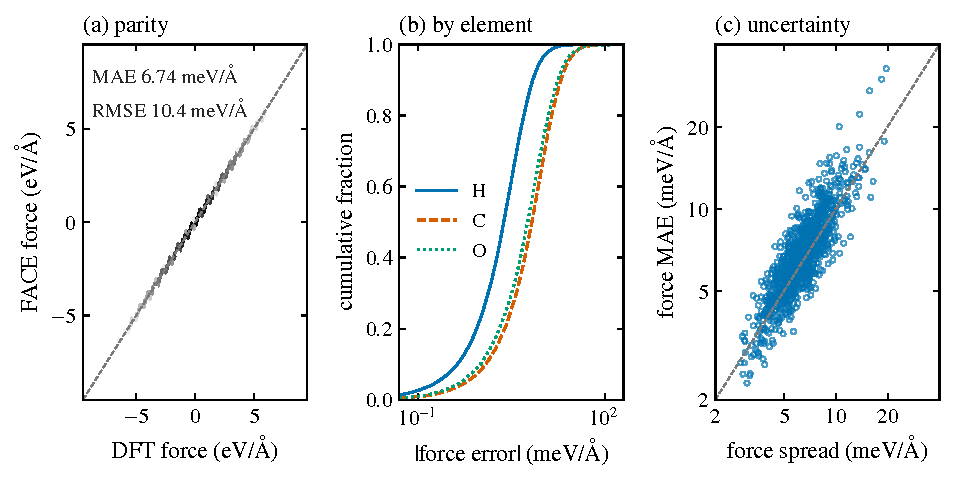
\includegraphics[width=\linewidth]{figures/fig_errors.pdf}
\caption{Error analysis on the aspirin test set (1000 structures). (a) Predicted versus reference force components
of the best single model (generation-4 \FACE-CP; logarithmic point density). (b) Cumulative distribution of
absolute force-component errors by element. (c) Per-structure force error of the five-model flagship ensemble
versus its force spread (Spearman 0.84); the dashed line marks equality.}
\label{fig:errors}
\end{figure}

\subsubsection{Uncertainty-gated distillation}
\label{sec:distillresults}
\emph{Distillation from thermal teacher dynamics brings a single model close to the best published accuracy.}
Figure~\ref{fig:distill}a shows why the distillation data must be thermal. Random Gaussian displacements of
0.02--0.06~\AA{} place structures where the teacher members disagree by 9.5--150~meV/\AA, because uncorrelated
displacements excite stiff modes far beyond thermal amplitude, whereas teacher MD at 500~K gives a spread of
6.9~meV/\AA, close to the 5.5~meV/\AA{} on the real test set; only 0.4--1.5\% of MD snapshots are rejected by the gate.
Figure~\ref{fig:distill}b,c and Table~\ref{tab:distill} show the effect of iterated distillation on a single \FACE-CP
model. Each generation reduced the force error, from 8.73~meV/\AA{} without distillation to 7.46, 7.04 and
6.97~meV/\AA{} in generations 1--3. A wider student was needed once the teacher (11 models, 2.55/6.53) surpassed the
published MACE accuracy, and the final energy-weighted fine-tune reduced the energy error by 9\% at a 0.6\% force
cost. The distilled generation-4 model (2.26/6.74) is within 3\% and 2\% of the published MACE result and better on
both errors than published NequIP, Allegro and TensorNet results. The flagship benefits from distillation as well
(3.13/8.04 from 3.13/9.08) while keeping its 5.7-fold speed advantage. Supplying more teacher data at the same
optimiser budget did not help (Table~S5), which suggests that the gain comes from the smoother labels on thermal
configurations near the training data rather than from the amount of data.

\begin{table}
\caption{Aspirin, single models, 1000 test structures (meV, meV/\AA). Published values are from different protocols.}
\label{tab:distill}
\begin{tabular}{lcc}
\toprule
model & $E$ MAE & $F$ MAE \\
\midrule
\FACE-CP, DFT data only, 400 epochs & 2.88 & 8.73 \\
generation 1 (7-model teacher), + DFT fine-tune & 2.71 & 7.46 \\
generation 2 (9-model teacher), + fine-tune & 2.69 & 7.04 \\
generation 3 (10-model teacher), + fine-tune & 2.50 & 6.97 \\
generation 4, $C=160$ student (11-model teacher), + fine-tune & 2.48 & 6.70 \\
generation 4, + energy-weighted fine-tune & \textbf{2.26} & \textbf{6.74} \\
\midrule
\FACE{} flagship, distilled + fine-tune (5.7$\times$ MACE-small speed) & 3.13 & 8.04 \\
\midrule
published TensorNet\cite{simeon2023tensornet} & 2.4 & 8.9 \\
published NequIP\cite{batzner2022} & 2.3 & 8.2 \\
published Allegro\cite{musaelian2023} & 2.3 & 7.3 \\
published MACE\cite{batatia2022mace} & 2.2 & 6.6 \\
published ViSNet$^a$\cite{wang2024visnet} & 1.93 & 6.59 \\
published QuinNet$^a$\cite{wang2023quinnet} & 2.11 & 6.20 \\
published GotenNet$^a$\cite{aykent2025gotennet} & 1.55 & 5.66 \\
\bottomrule
\multicolumn{3}{l}{\footnotesize $^a$converted from kcal/mol.} \\
\end{tabular}
\end{table}

\begin{figure}
\centering
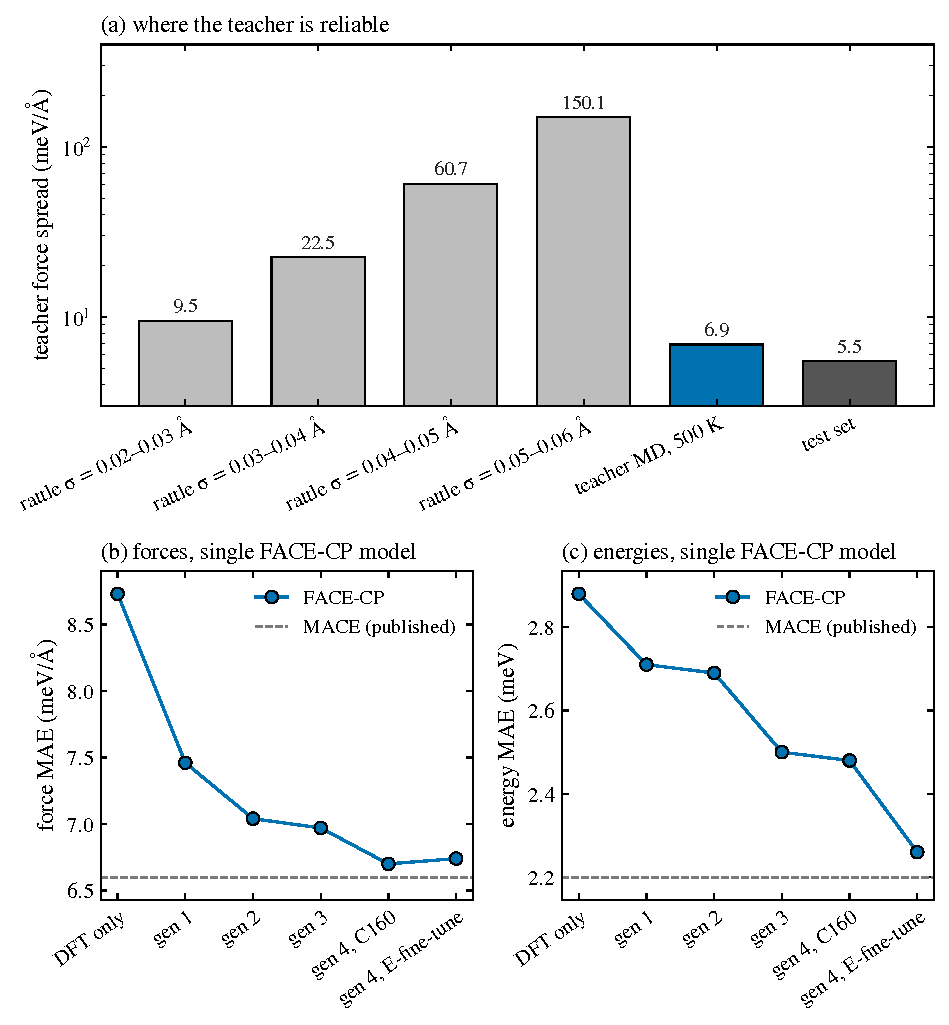
\includegraphics[width=\linewidth]{figures/fig_distillation.pdf}
\caption{(a) Teacher force spread on randomly rattled structures, on teacher-MD snapshots and on the real test set.
(b, c) Force and energy MAE of a single \FACE-CP model across distillation generations.}
\label{fig:distill}
\end{figure}

\subsubsection{Ethanol}
\emph{On ethanol the gap to published values is a matter of training protocol, not of the model.} On ethanol,
\FACE{} trails the published best values considerably more than on aspirin (single models 0.74--0.78/
4.7--4.9 vs 0.4/2.1). A control resolves this: MACE-small trained with the identical 400-epoch protocol reaches
1.11/6.76, so \FACE{} is about 30\% more accurate than MACE-small at equal training, and the gap to the published
number reflects the much larger float64 MACE configuration and its longer training. Distillation from a three-model
teacher improves the single \FACE-CP model to 0.68/4.22. Ethanol has a low-barrier methyl and hydroxyl rotation, and
its small size gives only eight neighbours per atom on average; both make it more sensitive to the description of
torsions than aspirin.

\subsection{Computational cost}
\subsubsection{Inference cost}
\emph{\FACE{} is several times cheaper than MACE at inference, but not in training.} Table~\ref{tab:speed} lists
the inference cost at 1,344 atoms. The flagship evaluates energy and forces in
33.3~$\mu$s per atom, 5.7 times faster than MACE-small and 10.9 times faster than MACE-medium. The fastest
configuration ($C=64$) is 6.3 times faster than MACE-small but less accurate on aspirin, and \FACE-CP trades a factor
of two in speed for higher accuracy. The published MACE configuration with 256 channels and $L=2$ needs
1.6~ms per atom at 168 atoms and does not fit in 12~GB at 1,344 atoms.

\begin{table}
\caption{Inference cost (energy + forces, float32, RTX 2000 Ada, 1,344 atoms) and training-step cost (batch of five
aspirin molecules, including second derivatives and the optimiser step, relative to MACE-small). Idle-GPU inference
values measured directly except those marked $^a$, derived from interleaved ratios to MACE-small under identical
load. ``vs MACE-s/-m'': inference speed-up relative to MACE-small/-medium; ``train step'': training-step time
relative to MACE-small.}
\label{tab:speed}
\small\setlength{\tabcolsep}{4pt}
\begin{tabular}{lrrrr}
\toprule
model & $\mu$s/atom & vs MACE-s & vs MACE-m & train step \\
\midrule
MACE-medium (128 ch)       & 361.5 & 0.53$\times$ & 1.0$\times$ & 1.35 \\
MACE-small (64 ch)         & 190.9 & 1.0$\times$  & 1.9$\times$ & 1.00 \\
\FACE{} flagship            & \textbf{33.3}  & \textbf{5.7$\times$} & \textbf{10.9$\times$} & 0.96 \\
\FACE{} $C=64$              & 30.4  & 6.3$\times$  & 11.9$\times$ & -- \\
\FACE-CP $C=96$             & $\approx$66$^a$ & 2.9$\times$ & 5.5$\times$ & 0.95 \\
\FACE-CP $C=160$            & $\approx$97$^a$ & 2.0$\times$ & 3.7$\times$ & 0.98 \\
MACE 256 ch, $L=2$         & 1634$^b$ & -- & -- & -- \\
\bottomrule
\multicolumn{5}{l}{\footnotesize $^b$measured at 168 atoms; out of memory at 1,344 atoms.} \\
\end{tabular}
\end{table}

\begin{figure}
\centering
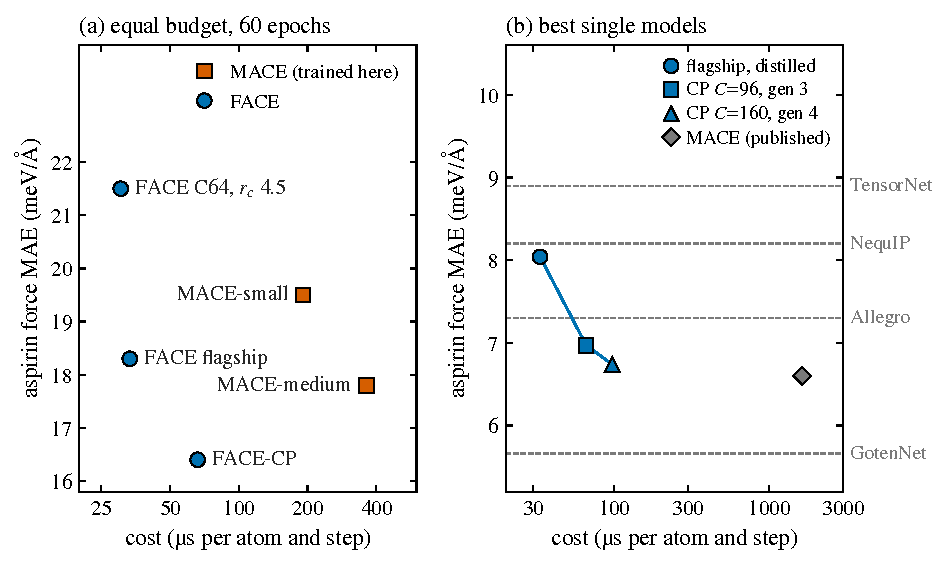
\includegraphics[width=\linewidth]{figures/fig_cost_accuracy.pdf}
\caption{Accuracy versus inference cost (energy and forces, $\mu$s per atom and step) on aspirin. (a) Equal 60-epoch
budget, all models trained here. (b) Best single models after long training and distillation versus published
long-training results (dashed lines). The published MACE configuration has 256 channels and $L=2$; its cost was
measured on our GPU at 168 atoms because it exceeds the memory limit at 1,344 atoms.}
\label{fig:cost}
\end{figure}

\subsubsection{Where the cost goes}
Profiling guided a sequence of exact, output-identical optimisations: replacing multi-operand einsums by broadcast
contractions (9--19$\times$ on those operations), performing the expansion from symmetric to full tensors as a general matrix multiplication (GEMM) with a
constant 0/1 matrix, pooling with one GEMM per rank on the small monomial array instead of slicing the large edge tensor, the
fused density kernel (forward 2.1$\times$ faster than PyTorch; backward 150~ms $\to$ 40~ms), the fused
node-algebra kernel (6.3$\times$), the constant-map transport and spline tables for narrow radial bases. The
flagship went from 1.6$\times$ to 5.7$\times$ the speed of MACE-small (Table~S3). Two negative results are worth
recording: mixed precision gave only 6--12\% because the remaining work is in memory-bound elementwise kernels, and
spline-compiled radial functions are slower than a small GEMM for wide radial heads. CUDA-graph capture of the full
energy and force evaluation, including the custom kernels, reduces launch overhead by 2.4$\times$ at 168 atoms but
has no effect at 4.5k atoms.

\subsubsection{System-size dependence}
Figure~\ref{fig:scaling} shows that the advantage depends on system size (Table~S7): the flagship is
2.3$\times$ faster than MACE-small at 168 atoms, 4.7$\times$ at 567, 5.6$\times$ at 1,344 and 5.4$\times$ at 2,625
atoms (2.4$\times$ to 3.2$\times$ for \FACE-CP). Small systems are limited by kernel-launch latency rather than
arithmetic, and CUDA-graph replay recovers a factor of 2.4 at 168 atoms. Above about 1,000 atoms the ratio is
constant, because both models then scale linearly with the number of atoms.

\begin{figure}
\centering
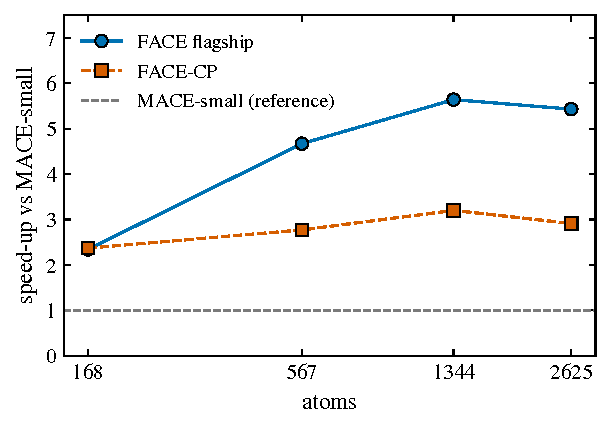
\includegraphics[width=0.62\linewidth]{figures/fig_scaling.pdf}
\caption{Inference speed-up relative to MACE-small as a function of system size (periodic aspirin boxes, energy and
forces, float32; medians of interleaved timing rounds).}
\label{fig:scaling}
\end{figure}

\subsubsection{Width and memory}
\label{sec:widthmem}
Figure~\ref{fig:widthmem}a tests the central claim of the cost model directly. At 1,344 atoms, widening the flagship
eightfold, from $C=32$ to $C=256$, increases its cost only 1.67-fold, from 0.16 to 0.27 of the cost of
MACE-small. Quadrupling the MACE width from 32 to 128 channels increases its cost 3.25-fold. \FACE-CP lies in between
(1.9-fold from $C=64$ to 160), as expected, because its edge work grows with $C$. Peak GPU memory for energy and forces
(Figure~\ref{fig:widthmem}b) grows linearly with the number of atoms for all models, at about 0.5~MB per atom for the
flagship, 1.3~MB for \FACE-CP and 2.0 and 3.9~MB for MACE with 64 and 128 channels. The flagship needs 3.5--3.9
times less memory than MACE-small at every size. At 4,536 atoms it uses 2.3~GB, whereas the 128-channel MACE no
longer fits within the 12~GB limit. Extrapolated linearly, a 12~GB budget holds about 23,000 atoms with the flagship
and about 6,000 with MACE-small, so the memory advantage extends the attainable system size on a single GPU by a
similar factor as the speed advantage. For molecular dynamics, the flagship's 33.3~$\mu$s per atom and step
corresponds to about 1~ns per day for 1,344 atoms with a 0.5~fs time step on this consumer GPU, excluding the
neighbour list.

\begin{figure}
\centering
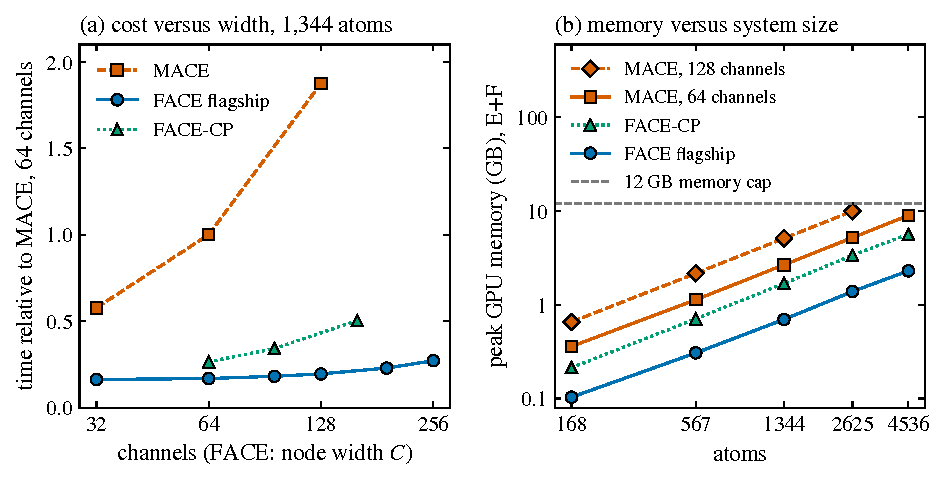
\includegraphics[width=\linewidth]{figures/fig_width_memory.pdf}
\caption{(a) Inference cost versus model width at 1,344 atoms, relative to MACE with 64 channels measured in the
same interleaved rounds; for \FACE{} the width is the node width $C$. (b) Peak GPU memory for one energy and force
evaluation versus system size; MACE with 128 channels exceeds the 12~GB cap at 4,536 atoms. Periodic aspirin boxes,
float32.}
\label{fig:widthmem}
\end{figure}

\subsubsection{Training cost}
Training is \emph{not} cheaper. A training step on five aspirin molecules, which requires second derivatives that
the fused kernels do not cover, costs 0.95--0.98 of a MACE-small step and 0.7 of a MACE-medium step
(Table~\ref{tab:speed} and Table~S8). A 400-epoch flagship run took 3.1~h on the same GPU. The distilled models of
Table~\ref{tab:distill} carry a further training overhead: generation 4 depends on seven 400-epoch teacher runs and
four earlier students and their fine-tunes, in total about $1.1\times10^6$ optimiser steps, or roughly 14 times the
training compute of a single 400-epoch model. Distillation therefore trades one-off training compute for inference
cost and accuracy.

\subsection{Training stability}
\label{sec:stability}
\emph{The divergences were caused by the weight parameterisation, not by the architecture.} Early versions diverged
on ethanol (NaN gradients from step 16 on every batch, with all weights finite). The
inputs of the invariant layer normalisation had grown to $10^{7}$ and $3\times10^{20}$, overflowing in the second
derivative. Layer normalisation is invariant to the overall scale of its input, so the optimiser can enlarge the
moments without changing the loss, and this scale direction reweights the body orders, because a $\nu$-body
invariant grows as the $(\nu-1)$-th power of the moment scale. Normalising the moments per atom stabilised training
but doubled the aspirin error, and data-calibrated fixed scales without layer normalisation diverged within 2--33
steps (Table~S2). A controlled probe at a constant learning rate located the cause in the weight parameterisation:
with the default parameterisation the relative change per step of the 1024-wide edge maps is about 30\%
(Section~\ref{sec:training}). With unit parameterisation the same architecture trained for 1500 steps at learning
rate 0.01 on ethanol without a single non-finite value (default parameterisation: first non-finite step 85), and the
optimal peak learning rate moved from 0.01 to 0.04. One of three ethanol seeds still diverged at learning rate 0.04
in a 60-epoch schedule; the recovery mechanism guards against this.

\subsection{Long-range interactions and charge}
\subsubsection{Benchmarks of Ko et al.}
\emph{Latent-charge electrostatics capture non-local charge effects that a local model cannot.}
Table~\ref{tab:lr} summarises the Ko et al.\ benchmarks. For C$_{10}$H$_2$/C$_{10}$H$_3^+$ with the default cutoff,
two message-passing steps reach about 10~\AA, comparable to the molecular length, and local and charge-equilibrated
models perform equally. With $r_c=3$~\AA{} (6~\AA{} receptive field, shorter than the 13~\AA{} chain), charge
equilibration halves both errors: the protonation state at one end of the chain changes the charge distribution at
the other, which only a non-local model can represent. For Ag$_3^\pm$, latent charges with the total charge as a
constraint reduce the energy error about 100-fold relative to the best local model. The two charge states were
sampled by separate MD and occupy mostly different geometries, so this set is not a same-geometry test; a local
model without equivariant saturation was numerically unstable on it (test error about 1.2~eV/atom). These trends
agree with the original study\cite{ko2021}, which reports energy errors of 0.6--2.0~eV/atom for a local
second-generation network and 0.3--1.2~meV/atom for the fourth-generation network on the DFT-optimised Ag$_3^\pm$
structures; because those values refer to optimised structures rather than to a test set, we do not compare them
numerically with Table~\ref{tab:lr}.

\subsubsection{Are the latent charges physical?}
The latent charges are never fitted to reference charges; they are intermediate variables determined by the
energy and forces. Figure~\ref{fig:charges} compares them with the Hirshfeld charges of the reference
calculations\cite{ko2021} on the 1000 test structures of each set. Over all atoms, the correlation is high for
Ag$_3^\pm$ (Pearson 0.96) and moderate for the carbon chains (0.68), but the overall value is dominated by the total
charge. Within each charge state the picture is mixed. For Ag$_3^+$ the latent charges follow the reference closely
(correlation 0.89, mean absolute deviation 0.011~$e$), and for the neutral C$_{10}$H$_2$ they reproduce the
atom-resolved Hirshfeld pattern (0.84). For Ag$_3^-$, however, the model distributes the excess
electron almost evenly (standard deviation 0.022~$e$ against 0.112~$e$ in the reference) and the within-state
correlation is negative ($-0.82$); for C$_{10}$H$_3^+$ it is absent (0.03). The latent charges therefore carry the
total-charge information that the energy requires, and in some systems they resemble a population analysis, but
they are not a substitute for one. Where physically meaningful charges or dipoles are needed, they should be added
to the loss, as in the fourth-generation networks\cite{ko2021}; the operator interface allows this without changes
to the model.

\begin{figure}
\centering
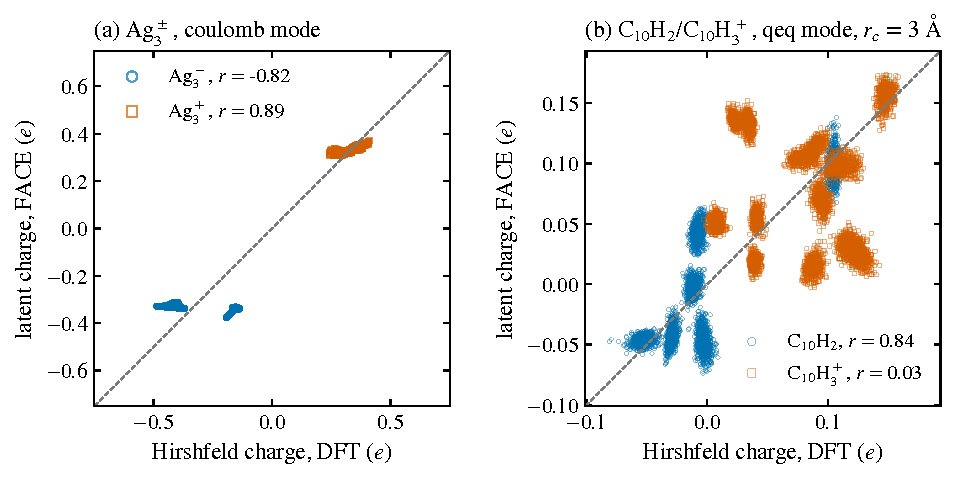
\includegraphics[width=\linewidth]{figures/fig_charges.pdf}
\caption{Latent charges predicted by \FACE{} versus Hirshfeld charges of the reference DFT calculations, which were
not used in training, for the 1000 test structures of (a) Ag$_3^\pm$ and (b) C$_{10}$H$_2$/C$_{10}$H$_3^+$
($r_c=3$~\AA). $r$: Pearson correlation within each charge state. Dashed line: equality.}
\label{fig:charges}
\end{figure}

\subsubsection{Cost of the physics operators}
The dispersion and ZBL operators were verified for correctness (symmetry, forces, periodicity) and cost only; none of
the data sets used here probes van der Waals binding or close nuclear contacts, so their benefit to accuracy remains
to be shown. Their cost was measured against the local flagship with fused kernels, interleaving all variants in
the same timing rounds (Table~S10). All three operators together add 23\% to the cost at 4,536 atoms, 28\% at 2,625,
44\% at 1,344 and 81\% at 567 atoms. Dispersion adds 9--12\% at every size, because its 10~\AA{} pair list is
several times longer than the model's neighbour list, and ZBL adds 2--8\%. The electrostatic operator dominates in
small systems: it adds 62\% at 567 atoms but only 12\% at 4,536 atoms, because the charge-grid and Fourier-transform
steps of SPME carry a fixed cost that is large compared with the fast local model when there are few atoms. The
operators are therefore affordable for large systems, but a substantial fraction of the cost for small ones, and they
should be switched on only where the physics requires them.

\begin{table}
\caption{Long-range benchmarks (Ko et al.), 1000 test structures: energy MAE (meV/atom) / force MAE (meV/\AA).}
\label{tab:lr}
\begin{tabular}{lll}
\toprule
system & local \FACE{} & with latent charges \\
\midrule
C$_{10}$H$_2$/C$_{10}$H$_3^+$, $r_c=5$~\AA{} & 0.33 / 12.6 & 0.36 / 14.5 (qeq) \\
C$_{10}$H$_2$/C$_{10}$H$_3^+$, $r_c=3$~\AA{} & 0.71 / 32.8 & \textbf{0.37 / 17.4} (qeq) \\
Ag$_3^+$/Ag$_3^-$ & 214 / 440$^a$ & \textbf{1.94 / 9.7} (coulomb) \\
\bottomrule
\multicolumn{3}{l}{\footnotesize $^a$with equivariant saturation; without it training was numerically unstable.}
\end{tabular}
\end{table}

\subsection{Molecular dynamics}
\emph{All models are stable in molecular dynamics and reproduce the thermal structure of the reference.} Low test
errors do not guarantee stable dynamics\cite{fu2023forces,bigi2024darkside}, so all main models were run in
NVE dynamics. All conserved energy: 20~ps at 500~K, drift $3\times10^{-4}$~meV/atom/ps; 10~ps from 1000~K (mean
658~K), $9\times10^{-4}$~meV/atom/ps; the flagship with fused kernels and spline-compiled radial functions,
$-0.004$~meV/atom/ps; the distilled generation-3 model, 5~ps from 1000~K, $-0.002$~meV/atom/ps. No bonds broke in any
run. This contrasts with direct-force models, for which unstable NVE dynamics have been reported\cite{bigi2024darkside}.

Figure~\ref{fig:md} documents a longer test of the best distilled model. In 20~ps of NVE dynamics started at 500~K,
the total energy fluctuates by 0.06~meV/atom (standard deviation) around a drift of
$-0.004$~meV/atom/ps, while the potential energy fluctuates by 8.0~meV/atom. In 20~ps of Langevin
dynamics at 500~K, the distributions of all 210 interatomic distances agree with those of the rMD17 reference data,
which were sampled by ab initio MD at 500~K\cite{chmiela2017md17} (mean kinetic temperature after the first
picosecond: 509~K). The overlap of the two normalised distance histograms is 0.97, and the mean bond lengths agree
to within 0.01~\AA{} (C--H $+0.009$, C--C $+0.006$, C--O $-0.006$, O--H $+0.0004$~\AA), which is small compared with
their thermal widths of 0.03--0.10~\AA. The model therefore conserves energy in NVE dynamics and reproduces the
thermal structural ensemble of the reference.

\begin{figure}
\centering
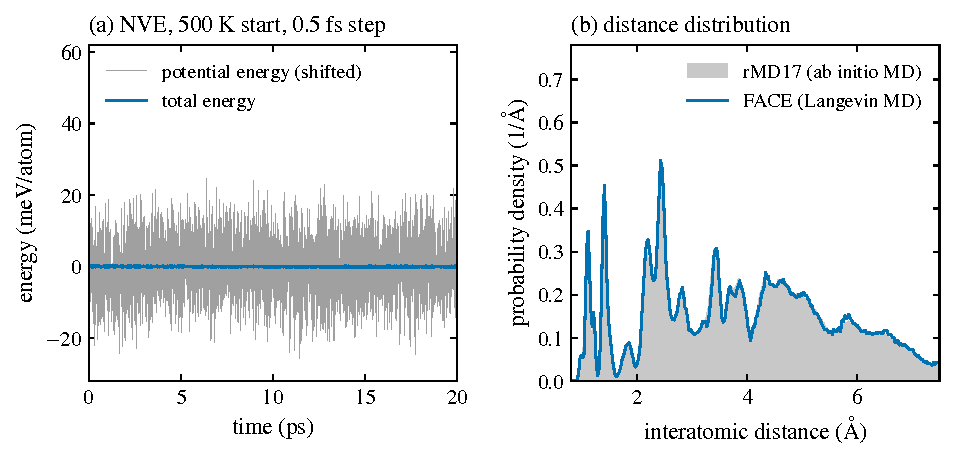
\includegraphics[width=\linewidth]{figures/fig_md.pdf}
\caption{Molecular dynamics of aspirin with the best distilled model. (a) Total and potential energy per atom in
20~ps of NVE dynamics from 500~K (0.5~fs time step); the potential energy is shifted for display. (b) Distribution
of all interatomic distances in Langevin dynamics at 500~K compared with the rMD17 reference data.}
\label{fig:md}
\end{figure}

%=====================================================================================================================
\section{Discussion}
\label{sec:discussion}

\subsection{Position among related models}
\FACE{} is closest to MTP and MACE. Like MTP, it uses Cartesian moment tensors of the bond directions; like MACE, it
builds the density from learned neighbour features and forms body-ordered products per atom over two
message-passing steps. Its differences are the factorisation of Equation~\ref{eq:effradial}, which moves the channel
dimension from the edges to the atoms; the transport of equivariant neighbour tensors through a constant map instead
of per-edge tensor products; and the evaluation of all products in symmetric Cartesian storage in fused kernels.
TensorNet and CACE also use Cartesian tensors but keep channel-wide tensors on each edge, and ICTP replaces
spherical by irreducible Cartesian tensor products, which are still evaluated on every edge. Allegro achieves its efficiency differently, by
restricting messages to edges and avoiding atom-to-atom message passing, which helps parallel scaling; the
factorisation in \FACE{} is compatible with that design in principle. The CP variant shows how the factorisation
interpolates between the two regimes: with a rank equal to the node width it recovers MACE's first-layer
density and costs about twice as much as the flagship, still three times less than MACE-small.

The results define when each configuration is useful. The flagship is the choice for long simulations where
inference cost dominates and an error of about 9~meV/\AA{} after standard training (8~meV/\AA{} after
distillation) is acceptable. \FACE-CP is about twice as expensive and reaches lower errors, in particular after
distillation. The ablations indicate that the accuracy of the flagship is limited by the rank $BK$ of the edge
factorisation, so the most effective way to trade cost for accuracy is to enlarge $B$ or $K_d$, not $C$.

\subsection{Limitations}
The theoretical foundation is not new; the novelty lies in the factorisation, the transport, the kernels, the
parameterisation and the training protocol. rMD17 is a saturated single-molecule benchmark. Materials, surfaces,
reactive chemistry and extrapolation tests (e.g.\ 3BPA\cite{kovacs2021}) were not performed, nor were the NaCl and
Au$_2$/MgO systems of Ko et al. All speed measurements use one consumer GPU in float32. The published MACE accuracy
was obtained in float64, and MACE was timed without the cuEquivariance kernels that are available on Linux, so the
speed ratios to MACE would shrink with those kernels; a comparison on multi-GPU or CPU hardware and in production
MD codes is outstanding. The advantage concerns inference: training steps cost about as much as MACE-small, and a
distilled model requires roughly an order of magnitude more training compute than a single model. Distillation was
demonstrated on aspirin and ethanol only and does not add information beyond the 950 reference structures; it
transfers the ensemble's averaged knowledge onto thermally sampled configurations. \FACE{} does not reach the most
accurate published aspirin results (ViSNet 1.93/6.59, QuinNet 2.11/6.20, GotenNet 1.55/5.66 meV, meV/\AA), whose
cost we have not measured. Several comparisons rest on single training runs, whose spread we quantified (about 3\%
at 400 epochs, 20--30\% at 60 epochs). The latent charges reproduce the total-charge partitioning but, without charge
reference data in the loss, not reliably the atomic charges themselves (Figure~\ref{fig:charges}). Finally,
ensembles are more expensive than single models; the uncertainty they
provide could instead be obtained from last-layer methods\cite{bigi2024llpr}.

\subsection{Outlook}
Three extensions follow directly from the results. First, fused kernels for the second-derivative pass would extend
the inference advantage to training. Second, the physics operators should be tested where they matter: ionic
materials, interfaces and molecular crystals, for which electrostatics and dispersion dominate the long-range
energy. Third, the factorisation leaves the per-atom part of the model free to grow, so multi-element systems, where
MACE-type models use element-dependent weights in the product basis, are a natural test of whether the edge rank or the
chemical complexity limits accuracy.

\section{Conclusions}
\FACE{} is a factorised Cartesian atomic cluster expansion in which the edge cost is independent of the feature width,
tensor transport is a constant linear map, and the body-ordered algebra runs in fused kernels. Physics operators for
electrostatics, dispersion and repulsion attach through one interface and add about 23\% to the cost of a
4,500-atom system. Unit parameterisation removes
the training divergences of this model class, and uncertainty-gated, iterated ensemble distillation with DFT-only
fine-tuning brings a single model within 3\% (energy) and 2\% (forces) of the published MACE aspirin result, at an
inference cost below that of a 64-channel MACE. The model is energy-conserving in long molecular dynamics and
reproduces the thermal structure of the reference data, and ensembles of the fast configuration provide calibrated
uncertainties. Natural next steps are fused kernels for the training backward pass, benchmarks on condensed-phase
and reactive systems where the physics operators matter, and implementation in production molecular-dynamics codes.

\begin{acknowledgement}
\Funding{} We thank the developers of rMD17, MACE, e3nn and ASE, and Ko et al., for making their data and
software openly available.
\end{acknowledgement}

\begin{suppinfo}
The Supporting Information is available free of charge on the ACS Publications website: architecture
development history and ablations; training-stability probe; kernel engineering; ensembles and seed variance;
additional distillation results; energy and force RMSE values; inference cost versus system size; training-step
cost; published reference values; hyperparameters; entries of the transport map; learning curves (PDF).
\end{suppinfo}

\section*{Author Information}
\textbf{Corresponding Author:} \AuthorName{} -- \AuthorAffiliation; ORCID \AuthorORCID; E-mail:
\AuthorEmail.\\
\textbf{Author Contributions:} \AuthorName{} conceived the study, designed and implemented the model, performed
all calculations and wrote the manuscript.\\
\textbf{Notes:} The author declares no competing financial interest.

\section*{Data and Software Availability}
The \FACE{} source code (Python/PyTorch with CUDA kernels compiled at run time through CuPy/NVRTC), the test suite,
all training logs, trained checkpoints, generated distillation data sets and the scripts that produce every table
and figure are publicly available under the MIT licence at \url{https://github.com/albert-hzbn/face-mlip}. Software versions: Python
3.12, PyTorch 2.6.0 (CUDA 12.4), CuPy 14.2, ASE 3.29\cite{larsen2017ase}, mace-torch 0.3.16, e3nn 0.4.4. The rMD17
data set is available from figshare (article 12672038); the data of Ko et al.\ from the Materials Cloud Archive
(record bk6kw-4b895).

\section*{Use of AI Tools}
An AI system (Claude Opus 5.5, Anthropic) assisted with the literature survey, the writing and debugging of the
software, running and analysing the experiments, and drafting and editing the manuscript and figures. All numerical
results were produced by the code in the accompanying repository and can be reproduced from it. The author reviewed
and edited all content and takes full responsibility for the work; the AI system is not an author.

\bibliography{references}

\end{document}
